%%% Example for master's thesis (in English)
\documentclass[dvipdfmx, english]{ampmt}             % pdflatex
%% \documentclass[dvipdfmx,english]{ampmt} % dvipdfmx

%%% Class options:
%%% chapter:   \chapter command is available (use report.cls).
%%% duplexing: Generate PDF for duplex printing.
%%% Options for article or report are also accepted.

%%% Title %%%%%%%%%%%%%%%%%%%%%%%%%%%%%%%%%%%%%%%%%%%%%%%%%%%%%%%%%%%%%%%%%%%%%%%
\title[Outlier detection technique to extract candidates of fraud from medical insurance claims]
      {Outlier detection technique to extract candidates of fraud from medical insurance claims}
      % [title for spine (option)]{title}
%%% Supervisors %%%%%%%%%%%%%%%%%%%%%%%%%%%%%%%%%%%%%%%%%%%%%%%%%%%%%%%%%%%%%%%%%
\supervisors{Aki-Hiro Sato}{Associate Professor}             % First supervisor  {name}{title}
            {}{} % Second supervisor {name}{title}
            {}{}                               % Third supervisor  {name}{title}
%%% Author %%%%%%%%%%%%%%%%%%%%%%%%%%%%%%%%%%%%%%%%%%%%%%%%%%%%%%%%%%%%%%%%%%%%%%
\author{Ryosuke Kawamori}
%%% Submission date %%%%%%%%%%%%%%%%%%%%%%%%%%%%%%%%%%%%%%%%%%%%%%%%%%%%%%%%%%%%%
\submissiondate{2019}{February}   % {year}{month}
%%% Number of output spines %%%%%%%%%%%%%%%%%%%%%%%%%%%%%%%%%%%%%%%%%%%%%%%%%%%%%
\def\numberofspines{1}
%%% Abstract %%%%%%%%%%%%%%%%%%%%%%%%%%%%%%%%%%%%%%%%%%%%%%%%%%%%%%%%%%%%%%%%%%%%
\abstract{%
This thesis proposes how to find fraudulent activities from data of medical insurance claims in an unsupervised way. Firstly, we split data into homogenous groups by the providers'{}
department, number of specialties, and their geographical location. If this is not accomplished, we may find providers performing rare operations, or providers in rural areas because of its variation in submitted charges.
Next, we apply the outlier detection method, One-SVM and LOF to these groups. Finally, we evaluate the effectiveness by using labels of providers who are excluded
because they committed fraud. The proposed method is above random and may be used as a first line of further investigation by specialties.

}
%%% Packages and definitions of your own macros %%%%%%%%%%%%%%%%%%%%%%%%%%%%%%%%%
\usepackage{amsmath,amssymb}
\usepackage{newtxtext,newtxmath} % Times font
\newcommand{\rme}{\mathrm{e}}


\usepackage{cite}
\usepackage{amsmath,amssymb,amsfonts}
\usepackage{algorithmic}
%\usepackage{graphicx}
\usepackage{textcomp}
\usepackage{xcolor}

%My definition and packages
\usepackage{comment}
\usepackage{tabularx}
\usepackage{bm}
\usepackage{here}
%\usepackage[dvipdfmx]{graphicx}
\usepackage{url}
\usepackage{longtable}
\usepackage{lscape}
\usepackage{ltablex}
\PassOptionsToPackage{hyphens}{url}
\usepackage{hyperref}

%\usepackage{showlabels}
%\usepackage[hang,small,bf]{caption}

\makeatletter
\let\MYcaption\@makecaption
\makeatother
\usepackage[subrefformat=parens]{subcaption}
%\captionsetup[sub]{parens}
\makeatletter
\let\@makecaption\MYcaption
\makeatother

\captionsetup{compatibility=false}
\newcommand{\Tabref}[1]{Tab.~\ref{#1}}
\newcommand{\Eqref}[1]{Eq. ~(\ref{#1})}
\newcommand{\Figref}[1]{Fig.~\ref{#1}}
\newcommand{\SubFigref}[1]{FIg.~(\ref{#1})}
\newcommand{\Secref}[1]{Section ~\ref{#1}}
\newcommand{\Appref}[1]{Appendix ~\ref{#1}}
\newcommand{\Listref}[1]{Listing ~\ref{#1}}



%ソースコード用
\usepackage{listings}
 
 \lstdefinelanguage{R}%
 {keywords={},
  otherkeywords={!,!=,~,$,*,\&,\%/\%,\%*\%,\%\%,<-,<<-,_,/},%
  alsoother={._$},%
  sensitive,%
  morecomment=[l]\#,%
  morestring=[d]",%
  morestring=[d]'% 2001 Robert Denham
 }%
 
\lstset{%
  language={R},
  basicstyle={\ttfamily},%
  identifierstyle={\small},%
  commentstyle={\small\itshape},%
  keywordstyle={\small\bfseries},%
  ndkeywordstyle={\small},%
  stringstyle={\small\ttfamily},
  frame={tb},
  breaklines=true,
  numbers=left,%
  xrightmargin=0zw,%
  xleftmargin=3zw,%
  numberstyle={\scriptsize},%
  stepnumber=1,
  numbersep=1zw,%
  lineskip=-0.5ex%
  basicstyle={\ttfamily},
  columns=[l]{fullflexible},
  lineskip=-0.5zw
}


%%% Control of output %%%%%%%%%%%%%%%%%%%%%%%%%%%%%%%%%%%%%%%%%%%%%%%%%%%%%%%%%%%

%%% If you don't want to output body text, activate the next line.
%% \outputbodyfalse

%%% If you don't want to output covers at the end of PDF, activate the next line.
%% \outputcoverfalse

%%% If you don't want to output abstract for submission at the end of PDF,
%%% activate the next line.
%% \outputabstractforsubmissionfalse

%%% If you want to change the layout, use \geometry command provided by
%%% the geometry package.
%% \geometry{hmargin=3cm,vmargin=2cm}

\begin{document}
\ifoutputbody
%%% Inside cover, abstract and table of contents %%%%%%%%%%%%%%%%%%%%%%%%%%%%%%%%
\makeinsidecover                % Inside cover
\makeabstract                   % Abstract
\maketoc                        % Table of contents
\setcounter{page}{1}
%%% Body %%%%%%%%%%%%%%%%%%%%%%%%%%%%%%%%%%%%%%%%%%%%%%%%%%%%%%%%%%%%%%%%%%%%%%%%

\section{Introduction}
The National Health Care Anti-Fraud Association estimated that at least 3$\%$(60 billion USD) of US annual health care expenditures were lost owing to outright fraud \cite{Survey}. 
Because of the great attention being paid to the patient safety, expectations, satisfaction, and advances in technology, there have been increases in the costs, which leaves greater room for fraud to occur\cite{Dean}.
To provide quality and safe care to legitimate patients, fraud control systems are needed. As noted above, because of upcoming health care technologies, many kinds of health care methods are in use. This makes it difficult to detect outright fraud manually in the vast amount of claims.
Thus, fraud detection model were needed.  \par
To detect outliers from many kinds operations, we firstly construct vectors which denote features of healthcare provider. For example, each elements of the vector are gender of the healthcare providers, number of  each operation he or she operated or amount of money paid to the provider during some period. Next, we apply
some fraud detection model to this vector. As noted above, many kinds of healthcare methods are in use, this vector tend to be high dimension. To extract fraudulent activities from high dimensional feature vector, Van \cite{Van} used the quantile of each dimension. However, in the case of upcoding, providers submitted a lower amount for one operation and a higher amount for another operation. To cope with this situation, we need to take several dimensions into consideration simultaneously. Shin \cite{Shin} used a weighted quantile as a outlier score. In the national health care program, providers can execute approximately 7000 types of operations. Thus, it is difficult to mix these operations to calculate one score by the experts. If we have data that has information on fraud labeling, we can build a supervised model to predict fraudulent activities. However, this method needs time-consuming labeling by domain experts and may be unable to find new types of fraudulent activities that are not in the training data. 
\par
In our study, we aim to support finding providers that commit fraud by extracting possibly fraudulent cases and use this model as a first line of further investigation by specialists. Our method is applicable to unlabeled data and can be used to extract candidates of outright fraud from a large amount of data. First, we split the data into homogeneous groups because dealing with all data simultaneously is computationally intensive, and if we try to find outliers from all providers, we may only find rare providers and times of computation is very long. Next, we try to find abnormal patterns in these groups.
%We define the normal data points as the point in the region where most of the data live and the others as abnormal. 
We use a one-class support vector machine (One-SVM) \cite{OneSVM} and Local Outlier Factor (LOF)\cite{Breunig} to find abnormal points. The One-SVM estimates a function that is +1 in the region where most data points live and -1 in the other regions and LOF which calculates the ratio of density of the object and its surroundings. To evaluate our methodology we use the List of Excluded Individuals and Entities(LEIE)\cite{Leie}. The LEIE contains information of the individuals and the entities that are currently excluded from the participation in Medicare, Medicaid and all other Federal health care programs. Although all physicians in the LEIE are cannot be detected in practical application levels, the evaluation metrics are above random. Thus our methodology can be used as a first line of further investigation.
\par
In \Secref{sec:hcf-and-ex-works}, we note what is defined as health care fraud and existing works regarding health care fraud detection. In \Secref{sec:data}, we describe datasets we use in this study and show statistics about the healthcare payments. In \Secref{sec:method}, we outline outlier detection algorithms and evaluation metrics. In \Secref{sec:results}, we show the effectiveness of our methods. In \Secref{sec:conclusions}, we summarize our research and give possible future works.






\section{Health care fraud and Existing works}\label{sec:hcf-and-ex-works}

\subsection{Health care fraud}
According to the National Health Care Anti-Fraud Association (NHCAA) \cite{Nhcaa}, health care fraud is ``an intentional deception or misrepresentation that the individual or entity makes knowing that the misrepresentation could result in some unauthorized benefit to the individual, or the entity or to some other party''
\par
There are three parties that may commit fraud: (a) service providers including doctors, hospitals, ambulance companies, and laboratories; (b) insurance subscribers, including patients and patients’{} employers; and (c) insurance carriers, who receive regular premiums from their subscribers and pay health care costs on behalf of their subscribers, including government health departments and private insurance companies\cite{Survey}.

NHCAA highlights the type of frauds listed below:

\begin{enumerate}
\item	Billing for services, procedures and/or supplies that were never provided or performed
\item Intentionally misrepresenting any of the following, for purposes of obtaining a payment-or a greater payment-to which one is not entitled:
	\begin{itemize}
		\item The nature of services, procedures and/or supplies provided or performed;
		\item The dates on which services and/or treatments were rendered;
		\item The medical record of service and/or treatment provided;
		\item The condition treated or the diagnosis made;
		\item The charges for services, procedures and/or supplies provided or performed;
		\item The identity of the provider or the recipient of services, procedures and/or supplies.
	\end{itemize}
\item The deliberate performance of medically unnecessary services for the purpose of financial gain.
\end{enumerate}

Furthermore, it is noted that there are two different types of fraud: ``hit-and-run“ and ``steal a little, all the time“\cite{Survey, Multidim}.``Hit-and-run“ perpetrators simply submit many fraudulent claims, receive payment, and disappear.``Steal a little, all the time“ perpetrators work to ensure fraud goes unnoticed and bill fraudulently over a long period of time.
Therefore, data, a data-preprocessing method, and a statistical model that detect fraudulent activity heavily depend on who commits fraud and what types of fraud we want to detect.

%So, here we see some works on the detection.

\subsection{Existing Works}

To combat fraud, there are three categories of intervention: Prevent, Detect, and Respond. These are listed in \Tabref{tb:intervention} \cite{Prevention}.
%Prevent means determining potential fraudulent providers and stopping them from committing fraud. For example, creating an anti-fraud culture and developing compliance systems are in this area.
Prevention interventions refer to ``the interventions that deter potential fraudsters from attempting fraud, and stopping a fraud attempt before the fraud is actually committed.'' For example, creating an anti-fraud culture and developing compliance systems are in this area.
%Detect means identifying fraudulent activity as quickly as possible after a fraud has been committed. For example, detecting fraud by data-mining methods and insider reporting systems are in this area.
Fraud detection involves ``identifying past and new cases of fraud as quickly as possible after a fraud has been committed.'' For example, detecting fraud by data-mining methods or insider reporting systems are in this area.
Response means ``administrative and legal actions based on the detection and investigation of the fraudulent cases in order to redress the lost money, fine the fraudsters, and sanction legal punishments to prevent future fraud.''
For example, changing and improving a system or law enforcement initiatives so that the chance of future fraud is reduced are in this area.
Most of the existing works focus on the effectiveness of detection\cite{NoEvidence}. Our research is also categorized as detection. We
try a data extraction method before conducting a detailed analysis of the experts’ research. Here we see existing works regarding fraud detection.

\begin{table}[H]
\centering
\caption{Three categories of Interventions to combat fraud.}\label{tb:intervention}
\begin{tabularx}{\linewidth}{l X}
\hline \hline
 Category & \\
\hline
Prevention & Prevent instances of fraud and misconduct from occurring in the first place. \\
Detection & Detect instances of fraud and misconduct when they do occur. \\
Response & Respond appropriately and take corrective action when integrity breakdown arise. \\
   \hline
\end{tabularx}
\addtocounter{table}{-1}
\end{table}



\subsubsection*{Supervised method}
Supervised algorithms are used to categorize datasets into fraudulent cases and normal cases. 
Ortega and He used a neural network\cite{Ortega, Neuralnet} and Bonchi used a decision tree \cite{Bonchi}. These methods need target data, which is a records of activities that were detected as fraudulent by the specialists.
Richard\cite{RichardRF} used Random forest with respect to various undersampling ratio data of providers because the Medicare dataset is highly unbalanced, meaning that most of the providers are labeled normal and a tiny number of providers are labeled fraudulent. 
Richard\cite{RichardMultiple} combined three data sources of Medicare procedures and applied Logistic regression, Gradient boosting and Random forest. 

\subsubsection*{Unsupervised method}
Rasim\cite{TwoModels} used demographic information and a quantile as a fraudulent score.
Richard\cite{RichardUnsupervised} used an Isolation Forest, Local Outlier Factor, Unsupervised Random Forest, Autoencoder, and $k\--$Nearest Neighbor, and evaluated their methods using a label provided by NHCAA of a provider who committed fraud.
Van\cite{Van} used a more story-based method. For example, they used the deviations from a simple linear model between the total dollar amount reimbursed and the number of reimbursed claims of a provider. They also used the percentage of dental claims for a specific tooth code. This idea was based on a report that some dentists repeatedly made claims for the same set of procedures by changing patient IDs in order to reimburse as much as possible with the least effort involved. Seo\cite{Seo2017Identifying} constructed a graph where nodes represent provider and edges represent their similarities and apply a PageRank algorithm to the network. They defined the outliers as nodes that have different specialties from seed nodes of PageRank and have a high PageRank score. Ekina \cite{ekina2013application} used a Bayesian co-clustering method to simulated data, where the providers and the beneficiaries are represented as network nodes.

\subsection*{Others}
Pande\cite{Pande} outlined the characteristics of physicians who were convicted of fraud, the consequences of their convictions, and the proposed problems of policies against fraud.
Li \cite{Survey} gave a survey, which includes a background of the health care fraud, data management, 
,models to detect fraud, and their evaluation.








\section{Data}\label{sec:data}

\subsection{Description of datasets}
Here we describe datasets we use. In order to detect fraud in health care receipts submitted by physicians registered in the US, we used three types of data: Medicare Provider Utilization and Payment Data from 2014, Physician and Other Supplier (Physician and Other Supplier PUF) \cite{PhysiAndOther}, Full Replacement Monthly NPI file \cite{NpiFile}, and all US zip codes with their corresponding latitude and longitude coordinates processed by MABLE/Geocorr2K ver1.3.3\cite{GeoCor}.

The first set of data, Physician and Other Supplier PUF records, contains information on services and procedures provided to Medicare beneficiaries by physicians and other healthcare professionals. Each row records information on utilization, payment and submitted charges organized by their National Provider Identifier (NPI) and Healthcare Common Procedure Coding System (HCPCS) code. The Physician and Other Supplier PUF information has been made public for the period 2012 to 2016.
For the sake of simplicity, we use only data from 2015. This data consists of  9,497,892 records and is used to make physicians'{} feature vectors. Each row records how much money each provider submitted for each operation in a year \cite{Puf}. \Tabref{tb:payment} describes the columns of this data and \Tabref{tb:payment-ex} shows an 
example of this data. For example first row of \Tabref{tb:payment-ex} indicates that a provider whose NPI code is 101111 submitted 10 dollars on average for a service with an HCPCS code of 91312.
\par

The second data set is the full replacement monthly NPI file, includes 5,400,369 records and provides the specialties of the providers.  Each row records the specialties of each provider. For example, internal medicine is categorized under specialties such as addiction medicine and bariatric medicine.
\Tabref{tb:npi} describe the columns of this data and \Tabref{tb:npi-ex} shows the example of this data. For example, The first row of \Tabref{tb:npi-ex} indicates that a provider whose NPI code is 101111 has only one specialty with code 207X00000X.
\par

The third data set, US zip codes, has 43,723 records. Each row records the longitude and latitude of a US zip code. We use this data to calculate which grid square code\cite{ASato} each provider belongs to.
\Tabref{tb:zip-ex} shows an 
example of this data. For example, the first row of \Tabref{tb:zip-ex} indicates that the longitude and latitude of zip code: 01008 are -72.402004 and 42.277543 respectively. These three datasets have more columns, but the columns which we do not focus on are omitted.
\par

To evaluate our methodology, we use the List of Excluded Individuals and Entities (LEIE). LEIE contains information on individuals and entities that were excluded from participation in Medicare, Medicaid, and all other federal health care programs in the period from 1977 to 2018\cite{Leie}. This data contains 70,491 records. Each row records the excluded physicians, excluded date, and the reason for their exclusion. Because providers who commit fraud are considered to be excluded from registration after their illegal activity, we use 
the providers' label of which their exclusion dates are after 2015.

\Tabref{tb:leie} shows an example of the LEIE data. For example, the first row of \Tabref{tb:leie} indicates that the provider whose NPI code is 101111 was excluded from participation in Medicare on 19/04/2018, and the reason for the exclusion is code 1128b7. 
The reasons for exclusion have 22 types. All exclusion reasons are in \Appref{sec:exclusions}. We do not use excluded physicians' records that are not related to fraud such as physicians who are excluded by the failure to disclose required information.
We use only fraud-related and excluded physicians whose exclusion reasons are in \Tabref{tb:leie} as in \cite{TwoModels}. 

\begin{table}[H]
\centering
\caption{Part of column description of Medicare Provider Utilization and Payment Data\cite{Puf}\label{tb:payment}}
\begin{tabularx}{\linewidth}{lXlX}
  \hline \hline
ID & Explanation \\
  \hline
npi & National Provider Identifier (NPI) for the performing provider on the claim.  \\
  nppes\_provider\_zip & The provider's zip code, as reported in NPPES.  \\
  hcpcs\_code & HCPCS code used to identify the specific medical service furnished by the provider. \\
  nppes\_entity\_code & Type of entity reported in NPPES. An entity code of ‘I’ identifies providers registered as individuals and an entity type code of ‘O’ identifies providers registered as organizations. \\
  nppes\_provider\_gender & When the provider is registered in NPPES as an individual (entity typecode=‘I’), this is the provider’s gender. \\
  nppes\_provider\_state  & The state where the provider is located, as reported in NPPES. \\
  provider\_type & Derived from the provider specialty code reported on the claim. \\
   line\_srvc\_cnt & Number of services provided; note that the metrics used to count the number provided can vary from service to service. \\
   bene\_unique\_cnt & Number of distinct Medicare beneficiaries receiving the service.\\
   bene\_day\_srvc\_cnt  &Number of distinct Medicare beneficiary/per day services.\\
  average\_submitted\_chrg\_amt & Average of the charges that the provider submitted for the service. \\ 
  average\_medicare\_payment\_amt & Average amount that Medicare paid after deductible and coinsurance amounts have been deducted for the line item service. \\ \hline
\end{tabularx}
\addtocounter{table}{-1}
\end{table}


\begin{table}[H]
\centering
\caption{Part of column descriptions of Full Replacement Monthly NPI file.}
\label{tb:npi}
\begin{tabularx}{\linewidth}{ l X}
  \hline \hline
ID & Explanation \\
\hline
Npi & National Provider Identifier (NPI) for the performing provider on the claim. \\
  Healthcare Provider Taxonomy Code\_1 & first specialty of the provider indicated by the NPI code. \\
  Healthcare Provider Taxonomy Code\_2 & second specialty of provider indicated by the NPI code. \\ \hline
\end{tabularx}
\addtocounter{table}{-1}
\end{table}

\begin{table}[H]
\centering
\caption{Part of column descriptions of all US zip code with their corresponding latitude and longitude coordinates.}
\begin{tabular}{lll}
\hline
ID & Explanation \\
\hline
zip & Zip code indicated by 5 digits. \\
lon & Longitude of corresponding zip code. \\
lat & Latitude of corresponding zip code. \\
   \hline
\end{tabular}
\label{tb:zip}
\end{table}

\begin{table}[H]
\centering
\caption{Examples of Medicare Provider Utilization and Payment Data. The raw data contains 9,497,882 rows and  19 columns.}
\begin{tabular}{lllll}
  \hline \hline
Npi & hcpcs\_code &$\cdots$& average\_medicare\_submitted\_amount & line\_srvc\_cnt \\
  \hline
101111 & 91312  & $\cdots$ & 10 & 3 \\
  101111 & 91313  & $\cdots$ & 10 & 4 \\
  101111 & 91314 & $\cdots$ & 25 & 2 \\
  101112 & 91312  & $\cdots$ & 50 & 2 \\
   \hline
\end{tabular}
\label{tb:payment-ex}
\end{table}

\begin{table}[H]
\centering
\caption{Examples of Full Replacement Monthly NPI file. The raw data contains 5,400,369 rows and 15 columns.}
\begin{tabular}{llll}
  \hline \hline
npi & Healthcare Provider Taxonomy Code\_1 & Healthcare Provider Taxonomy Code\_2 & $\cdots$\\
  \hline
101111 & 207X00000X & NA & $\cdots$\\
  101112 & 207RC0000X & NA & $\cdots$\\
  101113 & 174400000X & 207RH0003X & $\cdots$\\
   \hline
\end{tabular}
\label{tb:npi-ex}
\end{table}


\begin{table}[H]
\centering
\caption{Examples of zip code to its longitude and latitude file. The raw data contains 43,723 rows and 7 columns.}
\begin{tabular}{lll}
  \hline \hline
zip & lon & lat \\
  \hline
01008 & -72.402003  & 42.277543 \\
 01008 & -72.954983  &42.184969 \\
  01010 & -72.204899  & 42.12831 \\ \hline
\end{tabular}
\label{tb:zip-ex}
\end{table}


\begin{table}[H]
\centering
\caption{Examples of the List of Excluded Individuals and Entities. The raw data contains 70,491 rows and 18 columns. 15 of 5 columns are omitted.}
\begin{tabular}{lll}
  \hline \hline
NPI & EXCLDATE & EXCLTYPE \\
  \hline
101111 & 20180419 & $1128b7$ \\
000000 & 19940524 & $1128b5$\\
 184783 & 20110818 & $1128a1$ \\
   \hline
\end{tabular}
\label{tb:leie}
\end{table}

\begin{table}[H]
\centering
\caption{Fraud-related reasons of exclusion.}
\begin{tabularx}{\linewidth}{lXlX}
  \hline \hline
EXCLTYPE & Amendment \\
  \hline
1128a1 & Conviction of program-related crimes. Minimum Period: 5 years& \\
1128a2 & Conviction relating to patient abuse or neglect. Minimum Period: 5 years& \\
 1128a3 & Felony conviction relating to health care fraud. Minimum Period: 5 years& \\
 1128b4 & Felony conviction relating to controlled substance. Minimum Period: 5 years& \\
   \hline
\end{tabularx}
\addtocounter{table}{-1}
\label{tb:exclusion}
\end{table}


\subsection{Data Combination}

We combine the three types of datasets (Medicare Provider Utilization and Payment Data, Full Replacement Monthly NPI, and zip code) as shown in \Figref{fig:datacomb}
We split data from the provider’s{} department, number of specialties, and location. We have two reasons for using this data-split method. First, handling all providers simultaneously is very time consuming because LOF has $O(n\log n)$ time complexity
on the low\--dimensional data and One-SVM algorithm has $O(n^3)$ computational complexity, where $n$ is the number of the data points. Even though we split the data, the complexity does no decrease in the order of $n$. They decrease to $O(n\log{\frac{n}{M}})$ and $O(\frac{n^{3}}{M^{2}})$, where $M$ is the number of data split. However the number of provider $n$ is limited, the reduce of the time is effective and this is effective when we use parallel computing. 
Second, the variance in the provider’s {} feature vectors come from the provider's {} types, specialties, geographical location, and so on. With regard to geographical variance, we can easily assume that the providers in urban areas file more claims because they have many patients. It is also pointed out that spending per Medicare beneficiary also has a high variance\cite{GeoHealth}. Thus, if we try to find fraudulent claims from all providers, we may find providers who have rare specialties or who are in rural areas. These are the reasons to split the data. To split the data by location, we calculated the first grid square code \cite{ASato} from their geographical locations (latitude and longitude) by converting their zip codes.

\begin{figure}[H]
\centerline{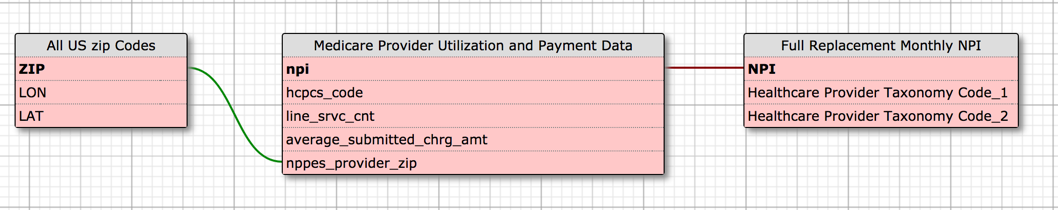
\includegraphics[scale=.8]{../img/datacomb.png}}
\caption{Conceptual illustration of data frame combination.}
\label{fig:datacomb}
\end{figure}

\subsection{Data understanding}\label{sec:data-undestanding}

\subsection*{Variation by provider specialty}
To see variation by provider type, we see histograms of the submitted amount of money. \Figref{fig:type-vari-his} shows part of the histograms of the total submitted amount of money by provider type.
The provider type has 141 kinds\footnote{Physician/General Practice, Physician/General Surgery, Physician/Allergy/ Immunology, Physician/Otolaryngology, Physician/Anesthesiology, Physician/Cardiovascular Disease (Cardiology), Physician/Dermatology, Physician/Family Practice, Physician/Interventional Pain Management, Physician/Gastroenterology, Physician/Internal Medicine, Physician/Osteopathic Manipulative Medicine, Physician/Neurology, Physician/Neurosurgery, Speech Language Pathologist, Physician/Obstetrics \& Gynecology, Physician/Hospice and Palliative Care, Physician/Ophthalmology, Oral Surgery (Dentist only), Physician/Orthopedic Surgery, Clinical Cardiac Electrophysiology, Physician/Pathology, Physician/Sports Medicine, Physician/Plastic and Reconstructive Surgery, Physician/Physical Medicine and Rehabilitation, Physician/Psychiatry, Physician/Geriatric Psychiatry, Physician/Colorectal Surgery (Proctology), Physician/Pulmonary Disease, Physician/Diagnostic Radiology, Anesthesiology Assistant, Physician/Thoracic Surgery, Physician/Urology, Chiropractic, Physician/Nuclear Medicine, Physician/Pediatric Medicine, Physician/Geriatric Medicine, Physician/Nephrology, Physician/Hand Surgery, Optometry, Certified Nurse Midwife, Certified Registered Nurse Anesthetist (CRNA), Physician/Infectious Disease, Mammography Center, Physician/Endocrinology, Hospital-Psychiatric Unit, Independent Diagnostic Testing Facility (IDTF), Podiatry, Ambulatory Surgical Center, Nurse Practitioner, Medical Supply Company with Orthotist, Medical Supply Company with Prosthetist, Medical Supply Company with Orthotist-Prosthetist, Other Medical Supply Company, Individual Certified Orthotist, Individual Certified Prosthetist, Individual Certified Prosthetist-Orthotist, Medical Supply Company with Pharmacist, Ambulance Service Provider, Public Health or Welfare Agency, Voluntary Health or Charitable Agency, Psychologist, Clinical, Portable X-Ray Supplier, Audiologist, Physical Therapist in Private Practice, Physician/Rheumatology, Occupational Therapist in Private Practice, Psychologist, Clinical, Clinical Laboratory, Clinic or Group Practice, Registered Dietitian or Nutrition Professional, Physician/Pain Management, Mass Immunizer Roster Biller, Radiation Therapy Center, Slide Preparation Facility, Physician/Peripheral Vascular Disease, Physician/Vascular Surgery, Physician/Cardiac Surgery, Physician/Addiction Medicine, Licensed Clinical Social Worker, Physician/Critical Care (Intensivists), Physician/Hematology, Physician/Hematology-Oncology, Physician/Preventive Medicine, Physician/Maxillofacial Surgery, Physician/Neuropsychiatry, All Other Suppliers, Unknown Supplier/Provider Specialty, Certified Clinical Nurse Specialist, Physician/Medical Oncology, Physician/Surgical Oncology, Physician/Radiation Oncology, Physician/Emergency Medicine, Physician/Interventional Radiology, Advance Diagnostic Imaging, Optician, Physician Assistant, Physician/Gynecological Oncology, Physician/Undefined Physician type, Hospital-General, Hospital-Acute Care, Hospital-Children’s (PPS excluded), Hospital-Long-Term (PPS excluded), Hospital-Psychiatric (PPS excluded), Hospital-Rehabilitation (PPS excluded), Hospital-Short-Term (General and Specialty), Hospital-Swing Bed Approved, Hospital-Rehabilitation Unit, Hospital-Specialty Hospital (cardiac, orthopedic, surgical), Critical Access Hospital, Skilled Nursing Facility, Intermediate Care Nursing Facility, Other Nursing Facility, Home Health Agency, Home Health Agency (Subunit), Pharmacy, Medical Supply Company with Respiratory Therapist, Department Store, Grocery Store, Indian Health Service facility, Oxygen supplier, Pedorthic personnel, Medical supply company with pedorthic personnel, Rehabilitation Agency, Organ Procurement Organization, Community Mental Health Center, Comprehensive Outpatient Rehabilitation Facility, End-Stage Renal Disease Facility, Federally Qualified Health Center, Hospice, Histocompatibility Laboratory, Outpatient Physical Therapy/Occupational Therapy/Speech Pathology Services, Religious Non-Medical Health Care Institution, Rural Health Clinic, Physician/Sleep Medicine, Physician/Interventional Cardiology, Dentist, Physician/Hospitalist, Physician/Advanced Heart Failure and Transplant Cardiology, Physician/Medical Toxicology, Hematopoietic Cell Transplantation and Cellular Therapy}\cite{Taxonomy}.
 Here we see part of the histograms of all provider types. We can easily see that different types of providers have very different histograms.
For example, Peripheral Vascular Disease has a high dollar amount. The mean amount is 719,014 USD. On the other hand, a Certified Nurse Midwife has a low dollar amount. The mean amount is 9,503 USD.

\begin{figure}[H]
	\begin{tabular}{ll}
	\begin{minipage}{.5\hsize}
	\centering
	\centerline{\includegraphics[scale=0.22]{../img/provider-type-variance/Internal-Medicine.pdf}}
%	\subcaption{Histogram of log of total submitted amount of money of providers whose speciality is internal medicine.}
	\subcaption{}\label{fig:internal}
	\end{minipage} 
      %---- 2番目の図 --------------------------
      \begin{minipage}{.5\hsize}
        \centering
        \centerline{\includegraphics[scale=0.22]{../img/provider-type-variance/Peripheral-Vascular-Disease.pdf}}
        	\subcaption{}\label{fig:peripheral}
%        \subcaption{Histogram of log of total submitted amount of money of providers whose speciality is peripheral vascular disease.}
      \end{minipage} \\
      %---3番目の図---------
       \begin{minipage}{.5\hsize}
        \centering
        \centerline{\includegraphics[scale=0.22]{../img/provider-type-variance/Addiction-Medicine.pdf}}
        \subcaption{}\label{fig:addiction}
%        \subcaption{Histogram of log of total submitted amount of money of providers whose speciality is addiction medicine.}
      \end{minipage} 
      %----4番目の図---------
       \begin{minipage}{.5\hsize}
        \centering
        \centerline{\includegraphics[scale=0.22]{../img/provider-type-variance/Certified-Nurse-Midwife.pdf}}
        \subcaption{}\label{fig:nurse}
%        \subcaption{Histogram of log of total submitted amount of money of providers whose speciality is certified nurse midwife.}
      \end{minipage} \\
      %---- 図はここまで ----------------------
    \end{tabular}
    \caption{\subref{fig:internal} depicts the histograms of the log of the total submitted amount of money of internal medicine. \subref{fig:peripheral} depicts that of Peripheral Vascular Disease. \subref{fig:addiction} depicts that of Addiction Medicine. \subref{fig:nurse} depicts that of Certified Nurse Midwife.}
    \label{fig:type-vari-his}
\end{figure}



%\begin{figure*}[ht]
%\centerline{\includegraphics[scale=0.47]{../img/provider-type-variance-limited.pdf}}
%\caption{Histograms of log of total submitted amount of money on each provider type.}
%\label{fig:type-vari-his}
%\end{figure*}


%\subsection*{Variation by providers' number of speciality}
%\Figref{fig:geo-vari-his} shows histogram of total submitted amount of money by providers' number of specialities. We can see that variation by provider's number is as high as by geograhical location and type of providers. So we may not need to split data by providers' number of speciality.

%\begin{figure}[H]
%\centerline{\includegraphics[scale=0.42]{../img/provider-spc-variance.pdf}}
%\caption{Histograms of lof of total submitted amount of money. X axis shows the mean of total submitted amount in each grid and Y axis shows the count of that value. We can see that the histogram has fat tail and the submitted amount of money is dependent on the area in the US.}
%\label{fig:spc-vari-his}
%\end{figure}



\subsection*{Geographical variance}
To see variation by geographical location, we computed the mean of the submitted amount of money in each grid square. The mean grid square statistics of the observed values $x_{ij}^{k}$, where $i$ is an index of the observed value, $j$ is a data feature, and $k$ is a grid square number, is defined as follows : \begin{equation}\label{eq:grid-stat}
m_{j}^{k}= \cfrac{1}{N_k} \sum_{i=1}^{N_{k}}x_{ij}^{k},
\end{equation}
%where $D_k$ is a set of index $i$ included in grid square $k$.
where $N_{k}$ is a number of observed points in the grid squre $k$.
\Figref{fig:geo-vari-map} shows the mean grid square of the total submitted amount of money on each grid $k$, and \Figref{fig:geo-vari-his} shows a histogram of the mean grid square of the total submitted amount of money. These figures indicate that there is strong geographical dependence with regard to the total submitted amount of money.

\begin{figure}[H]
\centerline{\includegraphics[scale=0.6]{../img/geographical-variance-map.pdf}}
\caption{Mean of the total submitted amount of money in each grid. Red corresponds to high submitted amount of money, and blue corresponds to the low submitted amount of money. We can see that the total submitted amount of money is high in urban areas and low in rural areas.}
\label{fig:geo-vari-map}
\end{figure}

\begin{figure}[H]
\centerline{\includegraphics[scale=0.6]{../img/geographical-variance-histogram.pdf}}
\caption{Histograms of the total submitted amount of money. X-axis shows the mean of total submitted amount in each grid. We can see that histogram has a fat tail, and the submitted amount of money is dependent on the area in the US.}
\label{fig:geo-vari-his}
\end{figure}




\subsection*{Variation by providers’{} number of specialties}
\Figref{fig:num-spc-vari} shows a histogram of the total submitted amount of money by the provider’{}s specialty. We can see that variations by the provider’s number of specialty is not as high as by the geographical location and the type of providers. Thus, we may not need to split data by the provider'{}s number of specialties.


\begin{figure*}[ht]
	\begin{tabular}{cc}
	\begin{minipage}{.5\hsize}
	\centering
	\centerline{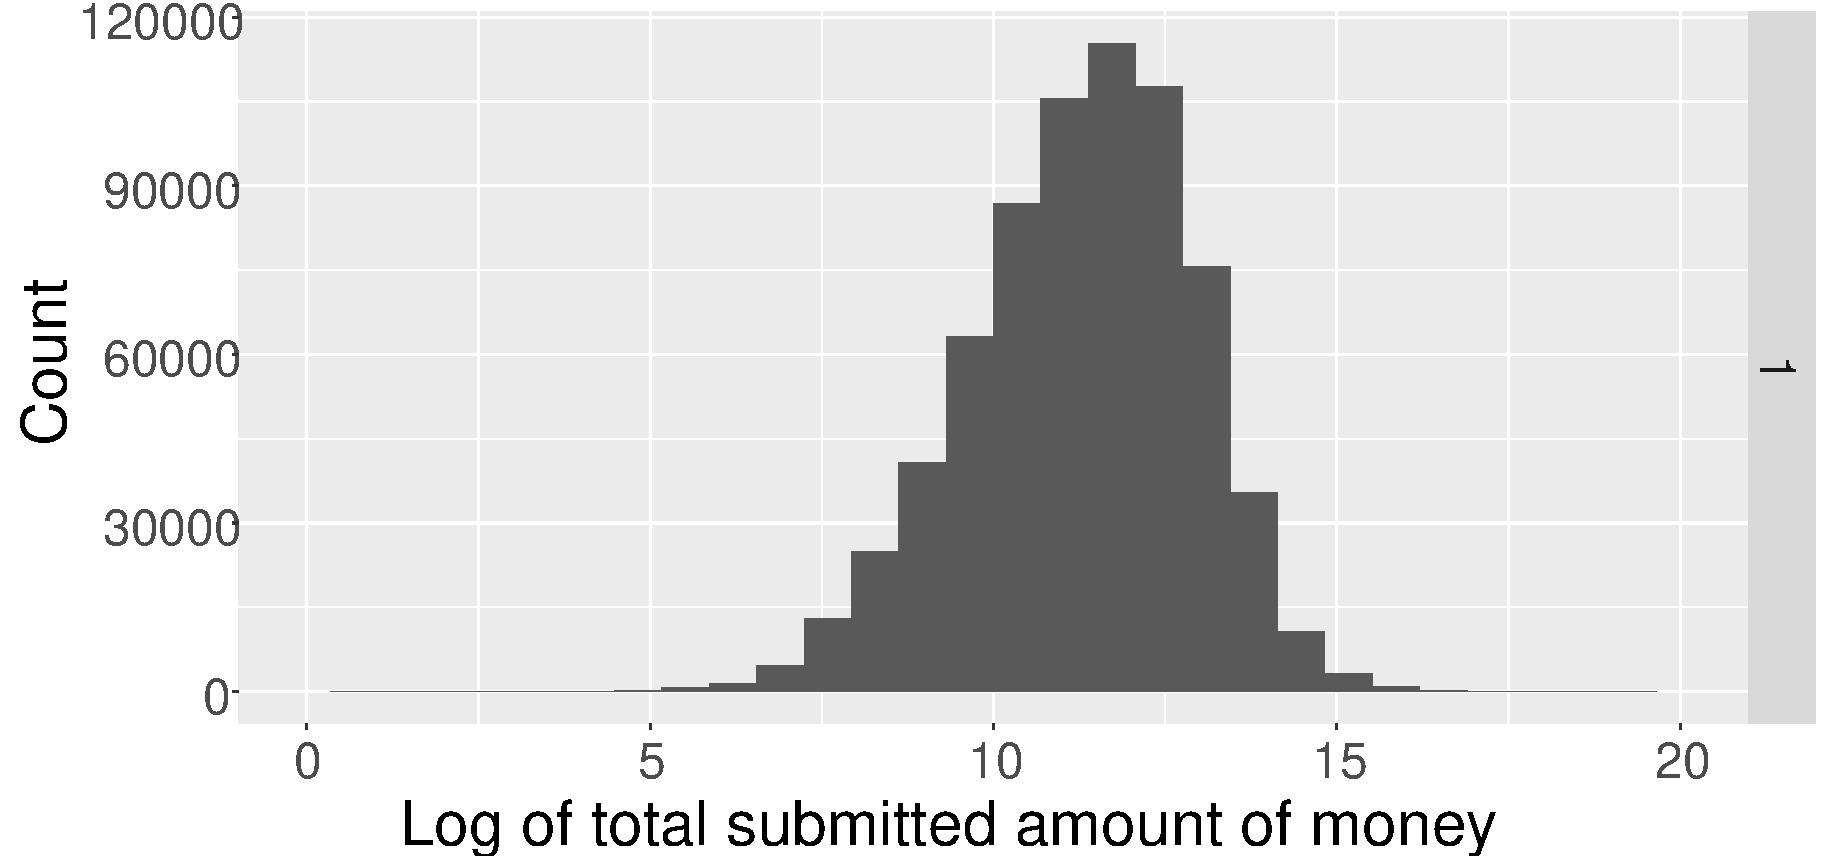
\includegraphics[scale=0.22]{../img/spc-type-variance/1.pdf}}
%	\subcaption{Histogram of log of total submitted amount of money of providers whose speciality is internal medicine.}
	\subcaption{}\label{fig:1}
	\end{minipage} 
      %---- 2番目の図 --------------------------
      \begin{minipage}{.5\hsize}
        \centering
        \centerline{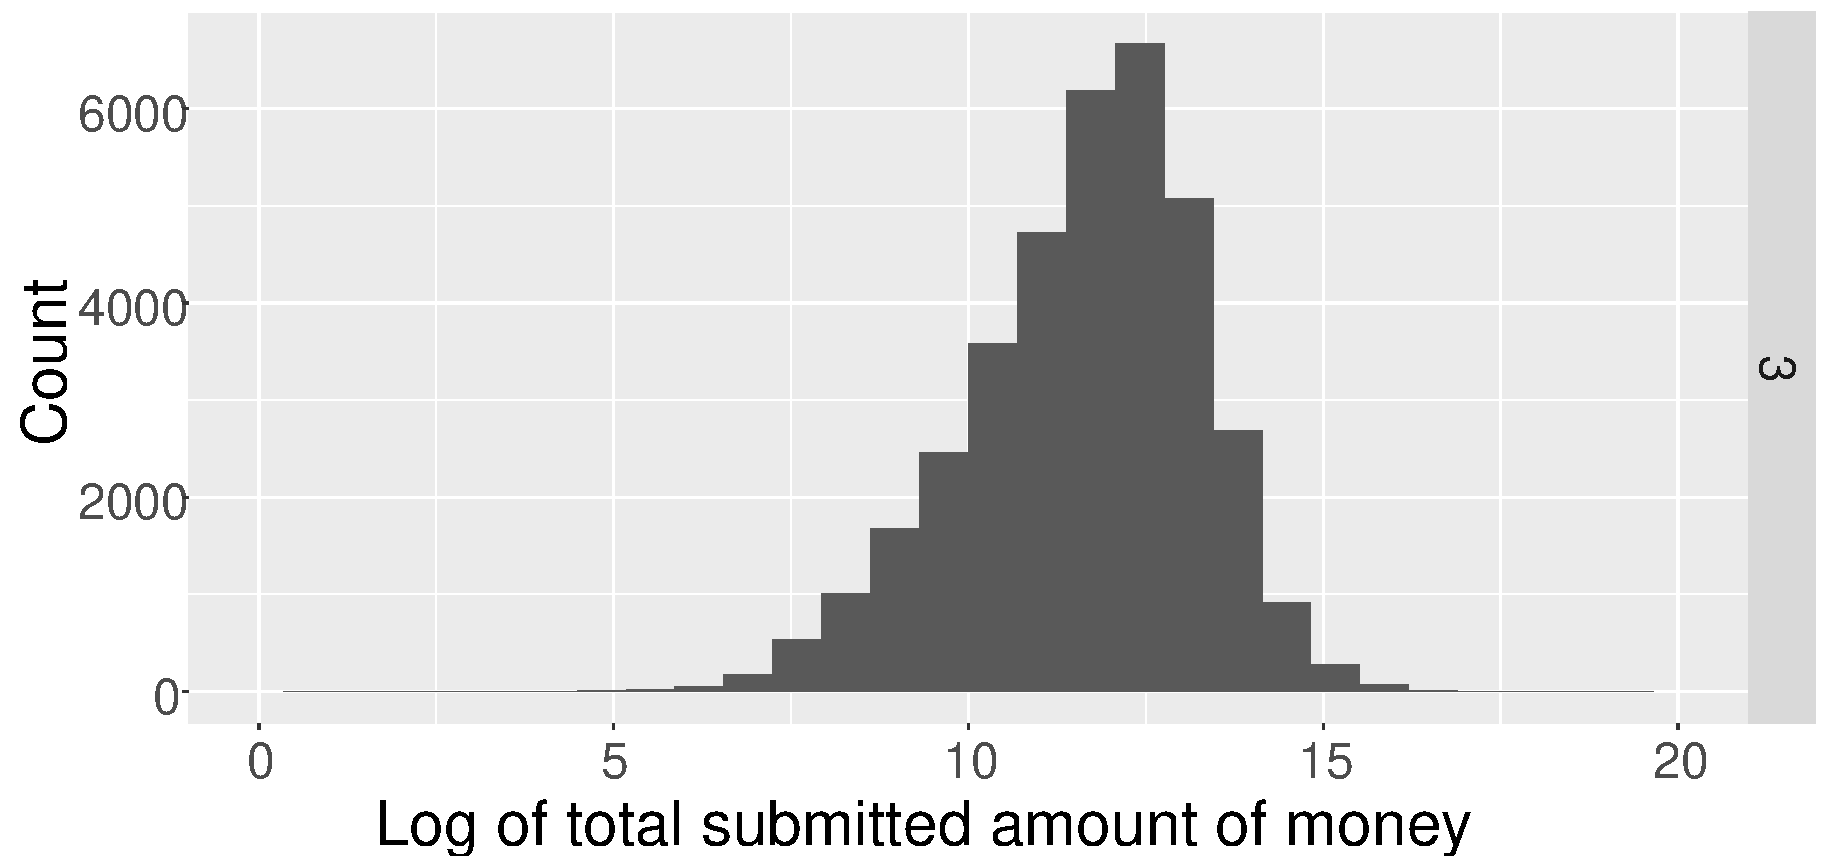
\includegraphics[scale=0.22]{../img/spc-type-variance/3.pdf}}
%        \subcaption{Histogram of log of total submitted amount of money of providers whose speciality is peripheral vascular disease.}
	\subcaption{}\label{fig:3}
      \end{minipage} \\
      %---3番目の図---------
       \begin{minipage}{.5\hsize}
        \centering
        \centerline{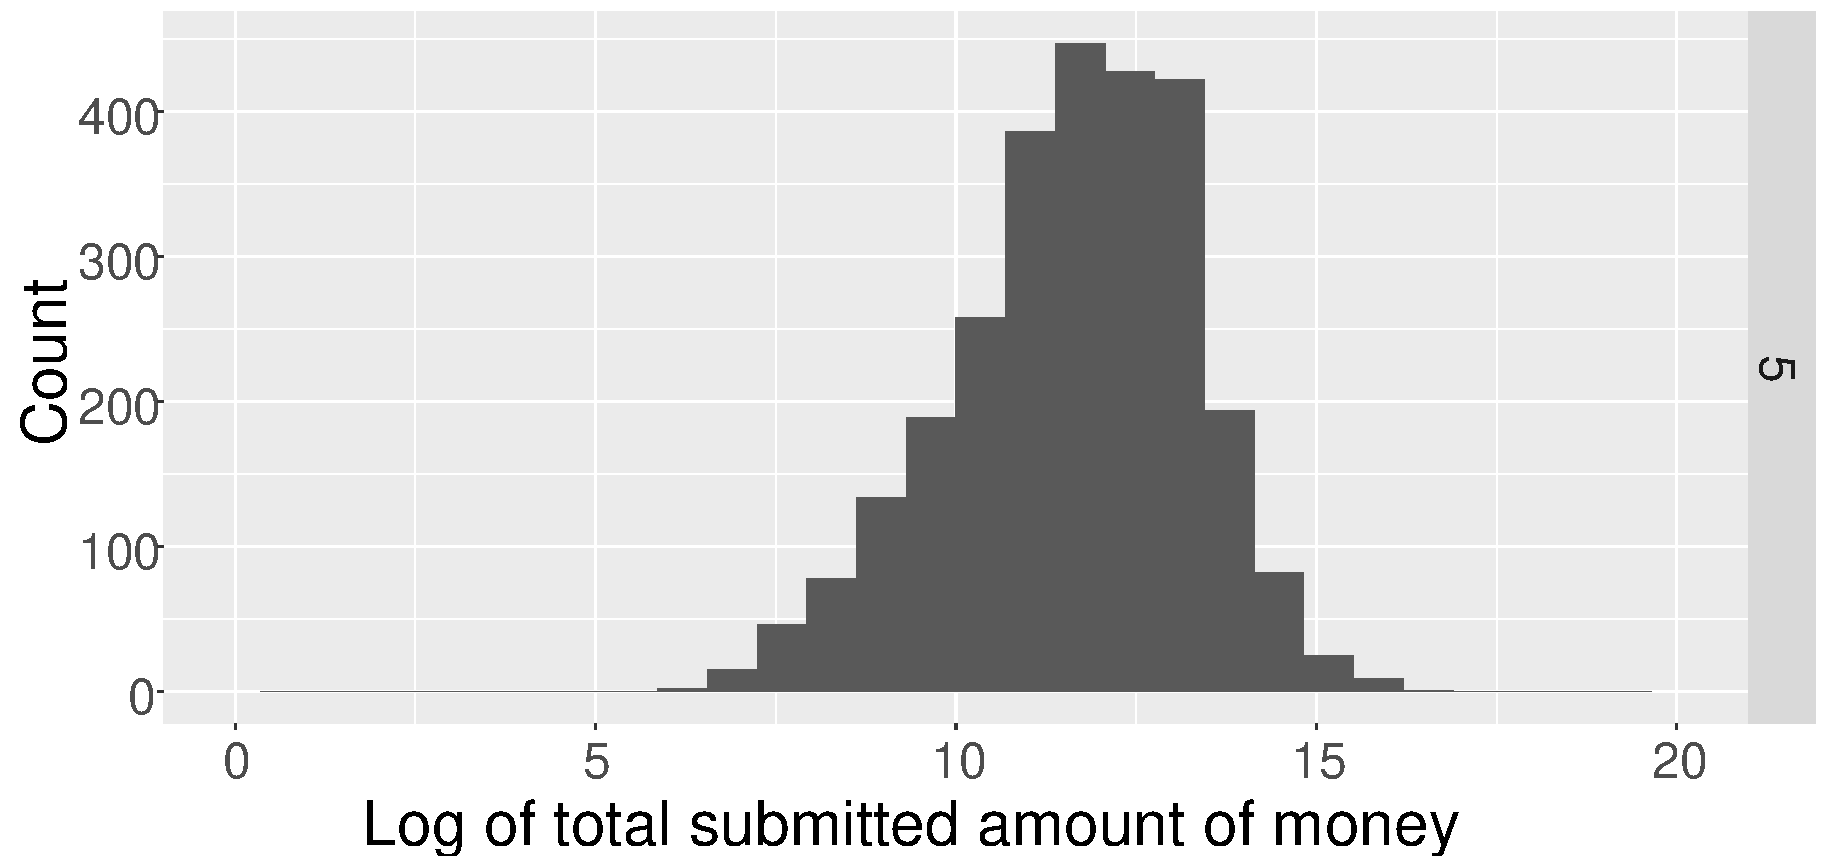
\includegraphics[scale=0.22]{../img/spc-type-variance/5.pdf}}
%        \subcaption{Histogram of log of total submitted amount of money of providers whose speciality is addiction medicine.}
	\subcaption{}\label{fig:5}
      \end{minipage} 
      %----4番目の図---------
       \begin{minipage}{.5\hsize}
        \centering
        \centerline{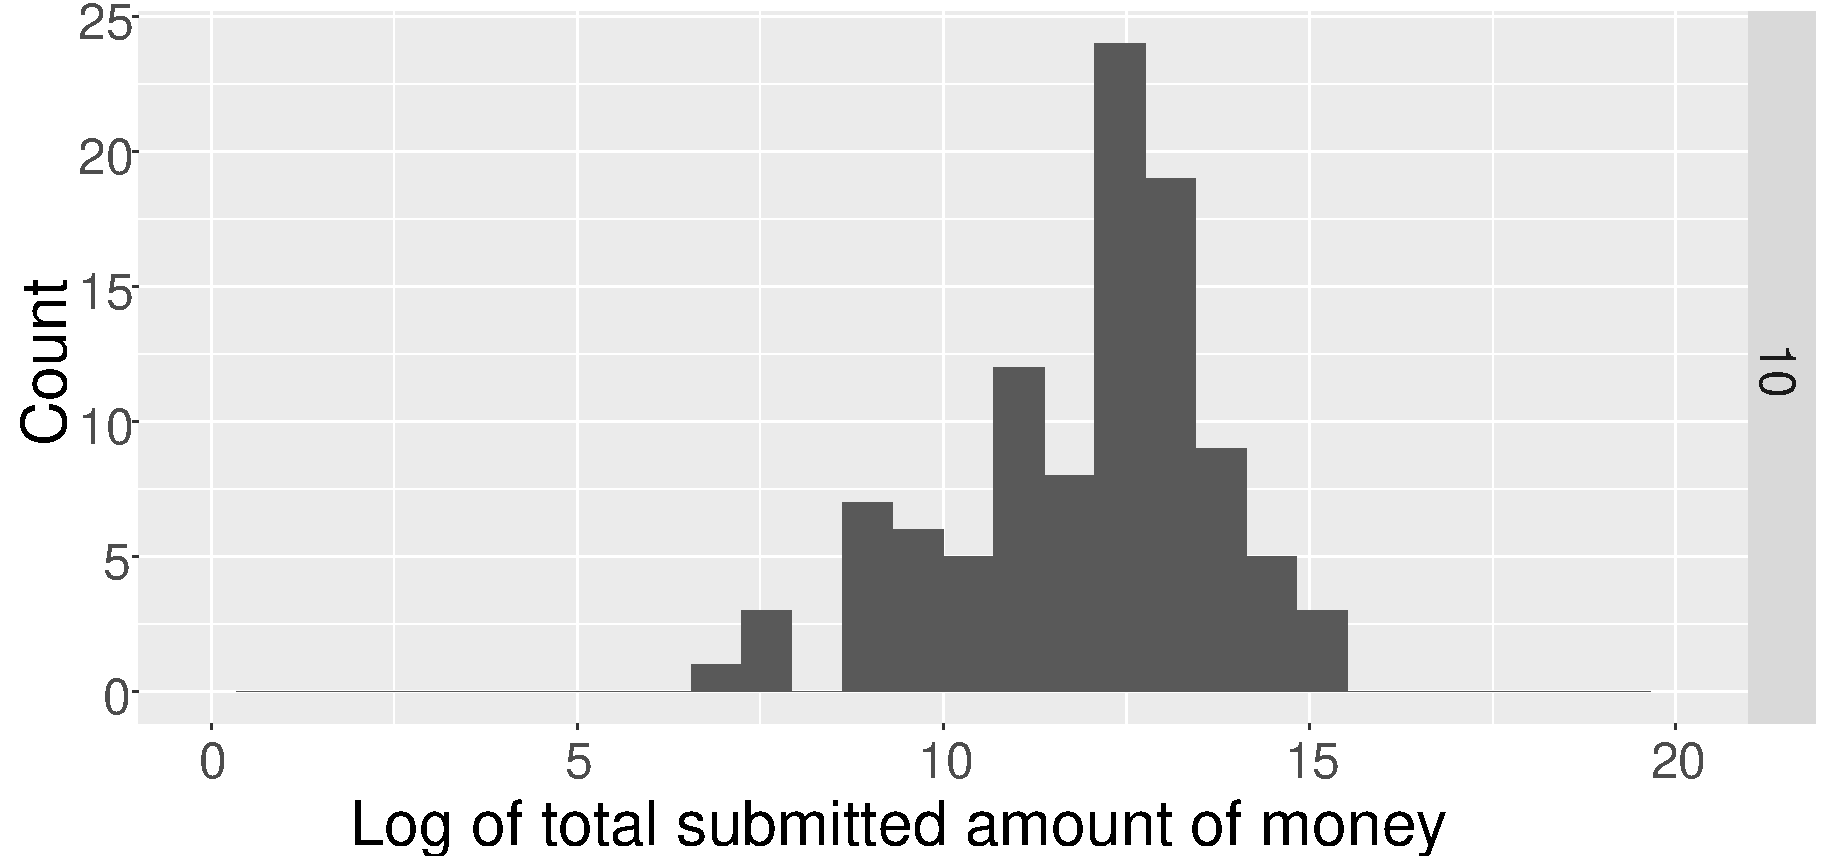
\includegraphics[scale=0.22]{../img/spc-type-variance/10.pdf}}
%        \subcaption{Histogram of log of total submitted amount of money of providers whose speciality is certified nurse midwife.}
	\subcaption{}\label{fig:10}
      \end{minipage} \\
      %---- 図はここまで ----------------------
    \end{tabular}
    
    
     \caption{\subref{fig:1} depicts histogram of log of total submitted amount of money by providers who have one specialty. \subref{fig:3} depicts that by providers who have 3 specialties. \subref{fig:5} depicts that by providers who have 5 specialties. \subref{fig:10} depicts that by providers who have 10 specialties.}
      \label{fig:num-spc-vari}
\end{figure*}



\section{Method}\label{sec:method}
\subsection{Subset of all data for evaluation}
We focus on providers in New York and California because we can obtain fraud label data to evaluate the efficiency of our methods due to strong fraud detection activities in these states.
Our main purpose is to extract candidates of fraud before specialists' investigations. Thus, in practical applications we should apply our extraction methods to the data from states where fraud enforcement is weak as well. However, we need metrics that evaluate our unsupervised strategy. We target individual providers in the states where fraud detection enforcement is strong. \Tabref{tb:subset} shows the descriptive statistics of our subset of all data used throughout our investigation.

\begin{table}[H]
\centering
\caption{Descriptive statistics of our subset of all data used throughout our investigation.}
\begin{tabular}{ll}
\hline \hline
Number of records & 1111686 \\
Number of providers & 123299 \\
Number of HCPCS codes performed & 4104\\
Number of providers who committed fraud & 46 \\
 \hline
\end{tabular}
\label{tb:subset}
\end{table}

\subsection{Feature engineering}

\subsection*{Feature engineering of existing works}

Richard \cite{RichardUnsupervised} calculated summary statistics of providers' procedure and construct provider\--level feature. They used the mean, median, max, min, sum, and standard deviation of 
%line\_srvc\_cnt, average\_medicare\_submitted\_amt, average\_medicare\_payment\_amt, bene\_uniuqe\_cnt 
the number of services provided, the number of distinct Medicare beneficiaries, the number of distinct Medicare beneficiary/per day services, the average of the Medicare allowed amount for the service, 
the average amount that Medicare paid after deductible and coinsurance amounts have been deducted for the line item service, the one-hot encoding of the providers'{}gender, and specialities. 
We call this feature engineering strategy STAT(statistics of all procedures).


\subsection*{Feature consisting of the submitted amount of each procedure}
From level 1: Single Claim, or Transaction to level 7: Multiparty, Criminal Conspiracies, there are seven levels of healthcare fraud control\cite{Survey, Multidim}. \Tabref{tb:level} shows these seven levels of focus. 
However, one row of our data describe what kind of procedure one provider operated in a year and we cannot obtain single claim, we can look at datasets only above or equal to level 3. Above level 3, for example, we can pay attention to the medical group whose providers belong to the same hospital. Here, for the sake of simplicity, we use level3b: One provider and all of its claims and related patients and do not use data above level3.


\begin{table}[H]
\centering
\caption{Levels of healthcare fraud control proposed by \cite{Survey}. This table was constructed by \cite{Multidim}.}
\begin{tabularx}{\linewidth}{llX}
  \hline \hline
  & & Level Focus \\ \hline
Level 1 & Single Claim, or Transaction &  The claim itself and the related provider and the patient.\\
  Level 2 & Patient/Provider & One patient, one provider, and all of their claims.\\
  Level 3 &  a. Patient & One patient and all of its claims and related providers.\\
  	      &  b. Provider & One provider and all of its claims and related patients. \\
  Level 4 & a. Insurer Policy / Provider & Patients that are covered by the same insurance policy and are targeted by one provider. \\
  	      & b. Patient / Provider Group & One patient being targeted by multiple providers within a practice. \\
  Level 5 & Insurer Policy / Provider Group & Patients with the same policy being targeted by multiple providers within a practice.\\
  Level 6 & a. Defined Patient Group & Groups of patients being targeted by providers. (e.g. patients living in the same location) \\
               &  b. Provider Group & Groups of providers targeting their patients. Groups can be providers within the same practice, clinics, hospitals, or other arrangements. \\
  Level 7 & Multiparty, Criminal Conspiracies & Multiparty conspiracies that could involve many relationships. \\
   \hline

\end{tabularx}
\label{tb:level}
\addtocounter{table}{-1}
\end{table}

We introduced grid separation \Eqref{eq:grid-stat} to calculate grid square statistics. This is an instance of splitting data in terms of geographical categories. Here let us introduce general data-split $k$, 
where $k$ is running from 1 to $M$. Let us define the $i$\--th data points: $\bm{x}_{i}^{k} = (x_{i1}^{k}, x_{i2}^{k}, \ldots, x_{il_{k}}^{k})$ as feature vector in $l_{k}$ dimensional space, where $k$ is a data-split index. The $j$\--th element of $\bm{x}_{i}^{k}$ is the log-transformed and normalized total submitted amount of money
for each service,
\begin{align}
 {x_{ij}^{k}}' &=  \ln⁡ \bigl((\mbox{Average of the charges that the provider submitted for the service of the }  j  \mbox{\--th hcpcs\_code} \nonumber \\ 
	& \mbox{of $i$\--th provider with data-split $k$}) \nonumber  \\ 
	 & \times  (\mbox{Number of services provided of the }  j  \mbox{\--th hcpcs\_code of $i$\--th provider with data-split $k$})\bigr), \nonumber \\
x_{ij}^{k} & =  \cfrac{{x_{ij}^{k}}'-m_{jk}}{\sigma_{jk}},
	\end{align}
where $m_j^{k}$ is a mean of $j$\--th data feature with data-split $k$ and $\sigma_j^{k}$  is the that of standard deviation.
\Tabref{tb:feature-ex} shows the providers’ features calculated from \Tabref{tb:payment-ex}.
We call this feature engineering strategy HCPCS (Each amount of HCPCS procedure).

\begin{table}[H]
\centering
\caption{Examples of feature-based data before log transformation and normalization.}
\begin{tabular}{ccccc}
  \hline \hline
NPI & $99312$ & $99313$ & $\cdots$ & $99314$ \\
  \hline
$10111111$ & $30$ & $40$ & $\cdots$ & $50$ \\
$10111112$ & $0$  & $0$ & $\cdots$ & $100$ \\
   \hline
\end{tabular}
\label{tb:feature-ex}
\end{table}


\subsection{Data-split method}
As noted in the previous section, the submitted amount of money have variances with regard to the physician's geographical location, type and number of specialities. 
We focus on physicians who have only one specialty, and we split the data by their location and specialty. We create a physician feature vector from this split-data frame and apply an outlier detection method. 
There are 6599 codes in HCPCS code set \cite{hcpcs} and the length feature vector is assumed to be 6599. However, some procedures are not performed when we focus on some split-data, then we omit these procedures from columns of the feature vector.

For example, the feature vector of the internal medicine physician with grid square code 306173 has $907$ elements, but
the feature vector of the same physicians with grid square code 304182 has 420 elements. We apply an outlier detection method to each split data item and combine the results into one data frame in order to calculate the evaluation metrics.
The conceptual image of this method is shown in \Figref{fig:data-split}. To check the efficiency of the data-split method based on geographical location, we compare three versions: PROVIDER (split only by physician’s specialty), GRID (split only by physician's grid square code), and  PROVIDER-GRID (split by physician’s specialty and grid square code).
We removed split data whose number of data points is smaller than 20. \Tabref{tb:Nk} shows the number of data-split $M$ of each data-split method of our subset.

\begin{figure}[H]
\centerline{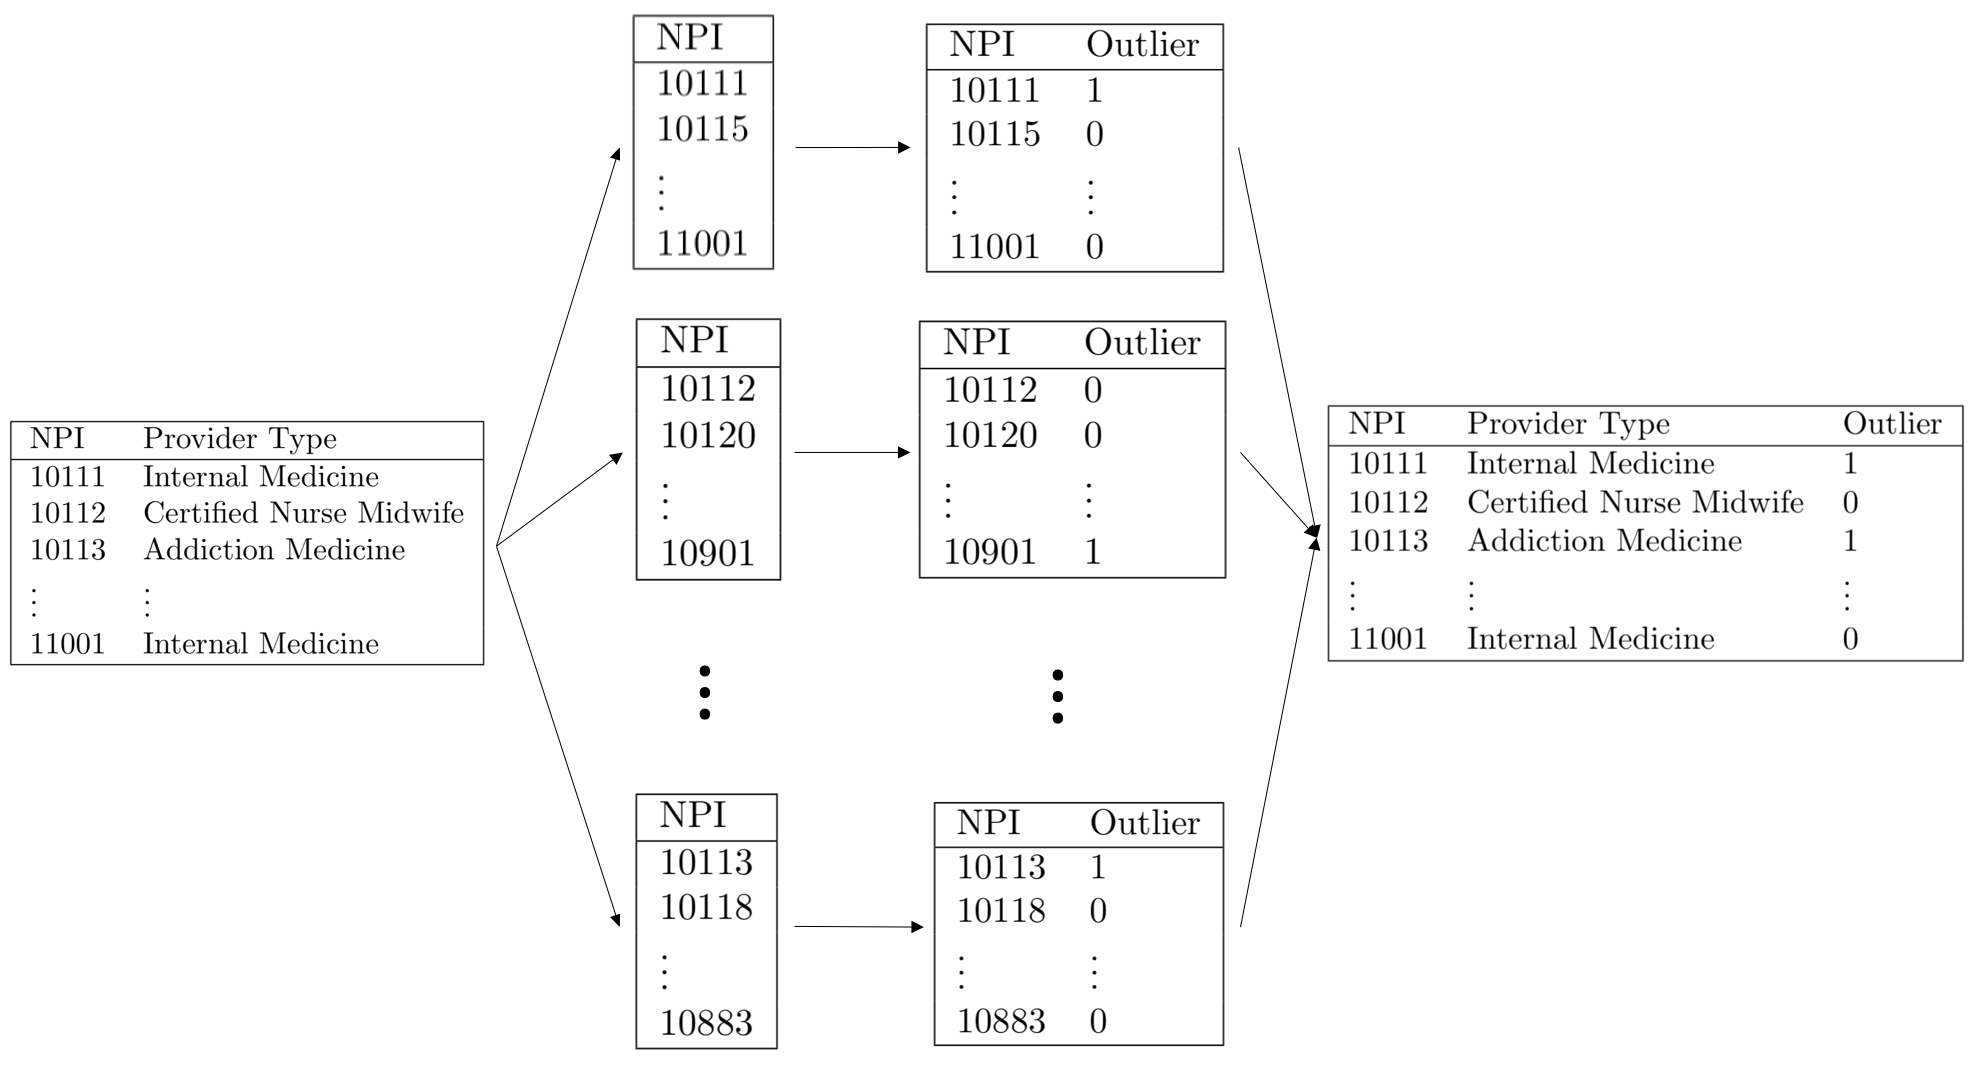
\includegraphics[scale=0.4]{../img/data-split.png}}
\caption{The conceptual illustration of the data-split method. We split data by their type and location, make physicians' feature vector from this split data frame and apply an outlier detection method.}
\label{fig:data-split}
\end{figure}

\begin{table}[H]
\centering
\caption{Number of data-split $M$ of each data-split method.}
\begin{tabular}{cc}
\hline \hline
Data-split method  & $M$ \\
\hline 
Provider & 66 \\
Mesh & 56 \\
Provider-Mesh & 967 \\
\hline
\end{tabular}
\label{tb:Nk}
\end{table}



\subsection{One Support Vector Machine}
Here we remove the index of data-split $k$ for clarity. Algorithms are applied in each data-separation $k$.
To detect fraudulent provider activity, we use a one-class support vector machine\cite{OneSVM} as an outlier extraction method. One support vector machine separates data from the origin to find the decision function that takes +1 in a region capturing most of the data points and -1 elsewhere. Mapping data into the feature space by function $\bm{\Phi}(\bm{x}): X \rightarrow F$, where $X$ is an input space and $F$ is a feature space that has an inner product and applying the one support vector machine in this space enable us to solve a nonlinear problem. One support vector machine is expressed as below,

\begin{flalign}
&\min_{\bm{w}\in F, \bm{\xi}\in \mathbb{R}^N, \rho \in \mathbb{R}} \cfrac{1}{2} ||\bm{w}||^2 + \cfrac{1}{\nu N} \sum_{i=1}^{N}\xi_{i}- \rho \nonumber \\
&\mbox{subject to} ⁡\qquad (\bm{w} , \bm{\Phi}(\bm{x}_i )) \geq \rho -\xi_i,\xi_i \geq 0.
\label{eq:one-svm}
\end{flalign}
Here, $||\cdot ||^{2}$ denotes the $l^{2}-$norm of a vector, $(\bm{w} , \bm{\Phi}(\bm{x}_i ))$ denotes the dot product of two vectors, $\bm{w}$ and $\bm{\Phi}(\bm{x}_i )$, in inner product space $F$, $N$ is a number of data points, and $\nu$ is a hyperparameter. The decision function is

\begin{equation}
\label{eq:f}
f(\bm{x}) = \operatorname{sgn}((\bm{w}, \bm{\Phi}(\bm{x}))-\rho),
\end{equation}
where
\begin{equation}
	\label{eq:sgn}
	\operatorname{sgn}(x) =
	\begin{cases}
	+1 \quad (x > 0)\\
	0  \quad (x = 0)\\
	-1 \quad (x < 0)
	\end{cases}.
\end{equation}
To solve main problem \Eqref{eq:one-svm} we derive dual problem. The Lagrange function is given as follows :
\begin{flalign}
L⁡(\bm{w}, \bm{\xi}, \rho, \bm{\alpha}, \bm{\beta}) &= \cfrac{1}{2} ||\bm{w}||^2 + \cfrac{1}{\nu N}  \sum_{i=1}^{N} \xi_i - \rho - \sum_{i=1}^{N} \alpha_i ((\bm{w} , \bm{\Phi}(\bm{x}_i))-\rho+\xi_i) - \sum_{i=1}^{N} \beta_i \xi_i .
\end{flalign}
where $\bm{\alpha} = (\alpha_{1}, \ldots, \alpha_{N})$ and $\bm{\beta} = (\beta_{1}, \ldots, \beta_{N})$, where $N$ is the number of data points, are dual variables. By taking derivative of the main variables $\bm{w}, \xi$, and $\rho$, we get,
\begin{flalign}
\label{eq:w}
\bm{w}-\sum_{i=1}^{N}\alpha_i \bm{\Phi}(\bm{x}_i) &=0, \\
\cfrac{1}{\nu l}-\alpha_i-\beta_i&=0,     \\
-1+\sum_{i=1}^{N}\alpha_i &= 0.
\end{flalign}
By using these equations, we get the dual of this program, given as follows : 
\begin{flalign}
\label{eq:dualpro}
&\max_{\bm{\alpha},\bm{\beta}⁡} \min_{\bm{w}, \bm{\xi}, \rho}  L(\bm{w}, \bm{\xi}, \rho, \bm{\alpha}, \bm{\beta}) =  \min_{\bm{\alpha}} \sum_{i=1}^{N}\sum_{j=1}^{N}\alpha_i \alpha_j (\bm{\Phi}(\bm{x}_i ), \bm{\Phi}(\bm{x}_j )) \nonumber \\
&\mbox{subject to} ⁡ \qquad 0 \leq \alpha_i \leq \cfrac{1}{\nu} , \quad \sum_{i=1}^{N}\alpha_i =1.
\end{flalign} 
By substituting \Eqref{eq:w} into \Eqref{eq:f}, we get
\begin{equation}
f(\bm{x}) =\operatorname{sgn}(\sum_{i=1}^{N}\alpha_i (\bm{\Phi}(\bm{x}_i ), \bm{\Phi}(\bm{x}))-\rho).
\end{equation}
Here we use Gaussian kernel, defined as
\begin{equation}
k(\bm{x},\bm{y})=(\bm{\Phi}(\bm{x}),\bm{\Phi}(\bm{y}))=e^{-\cfrac{||\bm{x}-\bm{y}||^2}{c}}.
\end{equation}
As we can see from the dual problem, we do not need to calculate $\bm{\Phi}(\bm{x})$ directly, and we only need the values of kernel function $k(\bm{x}_i, \bm{x}_j )$ when solving this problem. This technique is called the kernel method. We solve the dual problem expressed by \Eqref{eq:dualpro} using R package e1071 \cite{e}.  We set hyperparameters $c=\frac{1}{N}$ and $\nu=0.1$(package default). One support vector machine has two favorable properties. First, $\nu$ gives an upper bound of the ratio of the outliers, that is, the training points outside the estimated region. Second, there is a probabilistic guarantee that new points fall inside the estimated region.(For more details and proofs, see \cite{OneSVM}.)


\subsection{Local Outlier Factor}
LOF calculates the ratio of the density of the object and its surroundings.
The $k\--$distance of an object $p$ is defined as 
\begin{flalign}
	k\-- distance(p) = d(p,o),
\end{flalign}
 %$d(p,o) = \sqrt{\sum_{i}(p_{i}-o_{i})^{2}}$ 
where $d(p,o)$ is some distance measure between an object $p$ and an object $o$ such that:
\begin{enumerate}
	\item for at least $k$  objects $o'  \in D \setminus \{p\}$ it holds that $d(p,o') \leq d(p,o)$ and \\
	\item for at most $k-1$ objects $o'  \in D \setminus \{p\}$ it holds that $d(p,o') < d(p,o),$
\end{enumerate}
where $D$ represents the set of all data points. The $k\--$distance neighborhood of an object $p$ is defined as 
\begin{flalign}
	N_{k}(p) = \{q \in D\setminus {p} \mid d(p,q) \leq k\--distance(p)\}.
\end{flalign}
The local eachability distance of an object $p$ with respect to object $r$ is defined as
\begin{flalign}
	reach\--dist_{k}(p,r) = \max\{k\--distance(p), d(p,r)\}.
\end{flalign}
Local reachability density of an object $p$ is defined as 
\begin{flalign}
	lrd_{MinPts}(p) = \biggl\{ \cfrac{\sum_{q \in N_{MinPts}(p)} reach \-- dist_{MinPts}(p,q)}{\mid N_{MinPts}(p) \mid}  \biggr\}^{-1}.
\end{flalign}
This is the inverse of the mean of $reach \-- dist_{MinPts}$ from $p$ to its surroundings. So, this can be regarded as the density around point $p$.
Local outlier factor of an object $p$ is defined as the mean of the ratio of local density around $p$ and its surroundings $o$,  
\begin{flalign}
	LOF_{MinPts}(p) = \cfrac{\sum_{q \in N_{MinPts}(p)}  \cfrac{lrd_{MinPts}(q)}{lrd_{MinPts}(p)}}{\mid N_{MinPts}(p) \mid}
\end{flalign}
In our application, the data points are represented as vectora in $\mathbb{R}^{l}$ space and distance is Euclid distance, and set hyperparameter $MinPts=20$.
We use R package dbscan\cite{dbscan} to calculate LOF.



\subsection{Evaluation Metric}
We evaluate the effectiveness of data our data-extraction method using the true positive rate, the false negative rate, Receiver Operating Characteristic (ROC) curve, and Area Under Curve (AUC).
The true positive rate($TPR$) and the false negative rate ($FNR$) are defined as follows : 
\begin{flalign}
	TPR = \cfrac{TP}{TP+FN}, \\
	FNR = \cfrac{FN}{FN+TP},
\end{flalign}
where $TP$ is the number of physicians that are truly classified as fraudulent and $FN$ is the number of physicians that are falsely classified as normal.
The ROC curve created by plotting $TPR$ against the $FPR$ and the AUC is the area of the ROC curve. If physicians are randomly selected, the ROC curve is a straight line through two points $(0,0)$ and $(1,1)$ and the AUC is $0.5$.
If we can correctly classify physicians, the ROC curve is above that line and the AUC is above $0.5$. When applying One-SVM, we cannot get the outlier score but only labels and cannot draw the ROC curve in a standard way. However,
hyperparameter  $\nu$ works as an upper bound of the ratio of the outliers, thus, $TPR$  and $FPR$ assumed to increase as $\nu$ increases. We plot  $TPR$ against the $FPR$ with regard to 20 hyperparameter values $\nu$ running from 0.001 to 0.98. 
We regard this line as a ROC curve.


\section{Results}\label{sec:results}
%We focus on the result for healthcare receipts about internal medicine in 1st-level grid square 30617 and only one specialty:Internal Medicine.


%\subsection{Evaluation}

\subsection{One-SVM}

\Figref{fig:roc-svm} shows the ROC curve of the data-split method for PROVIDER and PROVIDER-GRID of STAT and HCPCS. All ROC curves are slightly above the straight line through points $(0,0)$ and $(1,1)$. 
However, they do not change much with respect to the data-split and the feature. Outliers found by One-SVM do not match with the fraudulent activities.


\begin{figure}[H]
\centerline{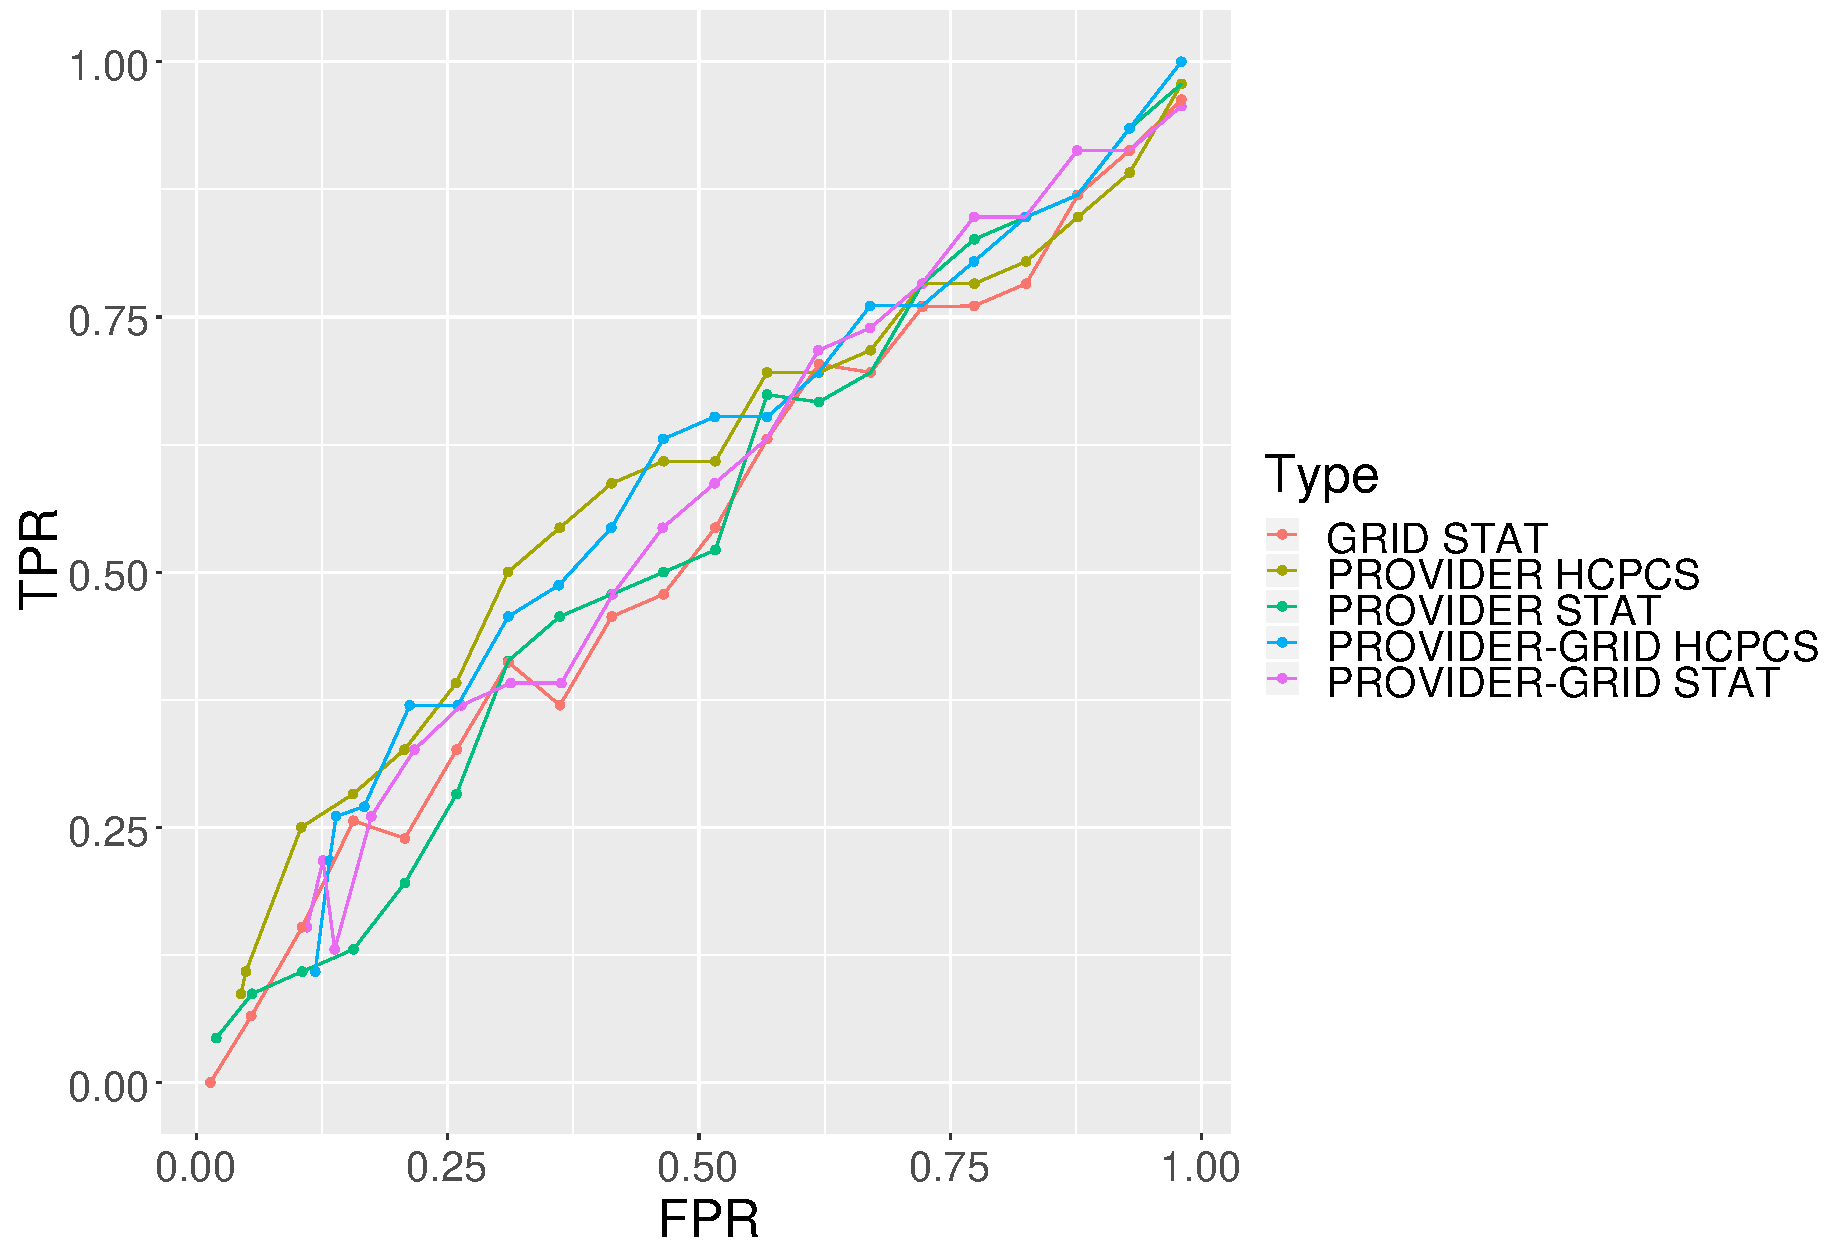
\includegraphics[scale=0.5]{../img/onesvm-roc.pdf}}
\caption{ROC curve of One-SVM with respect to the data-split: PROVIDER and PROVIDER-GRID of the feature: STAT and HCPCS. Type shows data-split method and how features are created.
%Red curve corresponds to data split method with provider of HCPCS. Green curve corresponds to data-split method for provider of Stat. 
%Bright green curve corresponds to data-split method for provider-mesh of HCPCS, and purple curve corresponds to data-split method for provider-mesh of Stat.
%Value side of points shows hyperparameter $\nu$ of one-SVM. 
X-axis shows true positive rate, and Y-axis shows false positive rate. All ROC curves are slightly above straight line through points $(0,0)$ and $(1,1)$. However, they do not change much 
with respect to data-splits and features.
}
\label{fig:roc-svm}
\end{figure}



\subsection{Local Outlier Factor}

\Figref{fig:roc-lof} shows the ROC curve of the data split: PROVIDER, GRID, and PROVIDER-GRID of the feature: STAT and HCPCS. All ROC curves are above the random extraction. 
All ROC curves are slightly above the straight line through points $(0,0)$ and $(1,1)$. In particular, data-split with data-split: PROVIDER and feature: HCPCS is the best of all.

\begin{figure}[H]
\centerline{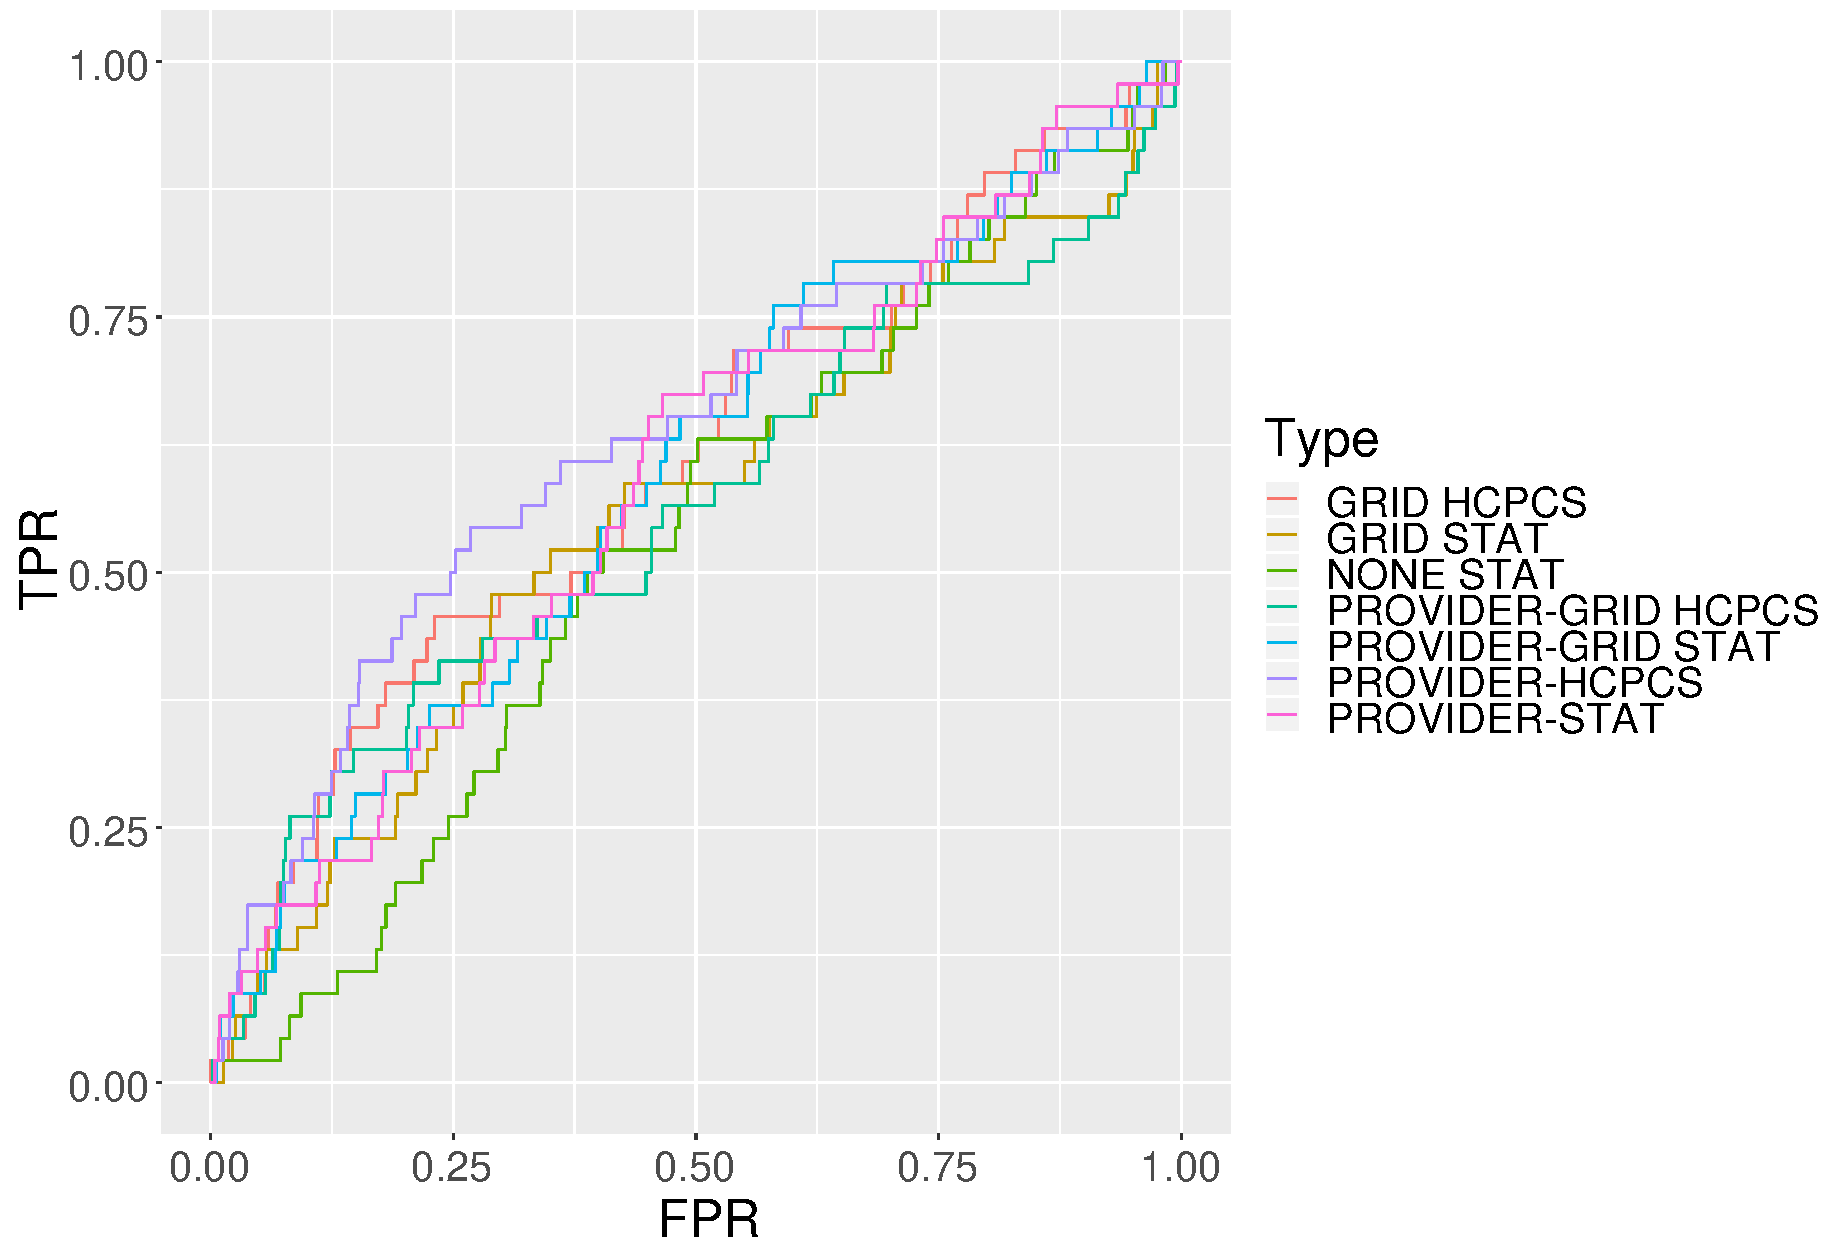
\includegraphics[scale=0.5]{../img/lof-roc.pdf}}
\caption{ROC curve of LOF with respect to data split: PROVIDER, GRID and PROVIDER-GRID of the feature: STAT and HCPCS. Type shows their data-split method and how their features are created.
%Value side of points shows hyperparameter $\nu$ of one-SVM. 
X-axis shows true positive rate, and Y-axis shows false positive rate. None means there was no data split. All ROC curves are slightly above straight line through points $(0,0)$ and $(1,1)$. In particular, data split for provider of feature with HCPCS had the best result.}
\label{fig:roc-lof}
\end{figure}


%\subsection*{Effect of data split method and feature engineering strategy}
%\Figref{fig:dc1-roc} shows the ROC curve of two feature engineering strategy STAT and PROC with data split method:DC1. \Figref{fig:dc2-roc} shows that with data split method:DC2.

%\begin{figure}[H]
%	\begin{tabular}{c}
%	\begin{minipage}{.9\hsize}
%	\centering
%	\centerline{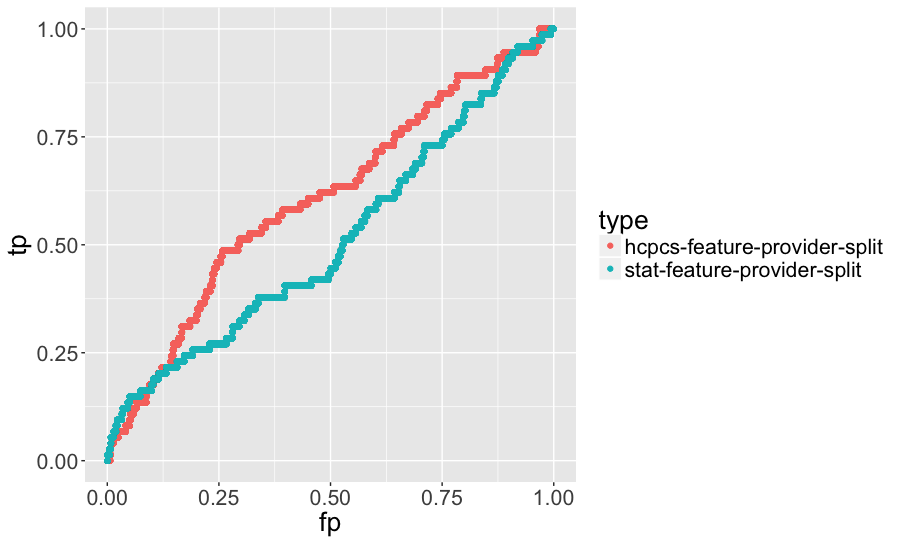
\includegraphics[scale=0.2]{../img/roc-provider-split.png}}
%	\subcaption{Histogram of log of total submitted amount of money of providers whose speciality is internal medicine.}
%	\subcaption{ROC curve of STAT(statistics of procedure feature) and PROC(each procedure feature) with data split method:SP1. }
%	\subcaption{ROC curve of two feature engineering strategy STAT. The red curve shows the feature engineering strategy, PROC:each procedure and the green curve shows the feature engineering strategy, STAT:statistics of all procedures.}
%	\label{fig:dc1-roc}
%	\end{minipage} \\
      %---- 2番目の図 --------------------------
 %     \begin{minipage}{.9\hsize}
   %     \centering
      %  \centerline{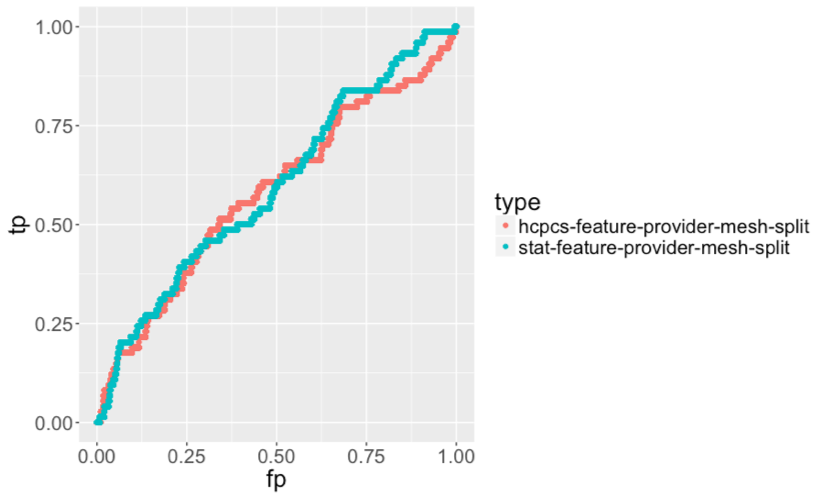
\includegraphics[scale=0.4]{../img/DC2-roc-feature.png}}
%        \subcaption{Histogram of log of total submitted amount of money of providers whose speciality is peripheral vascular disease.}
	%\subcaption{}
%        \label{fig:dc2-roc}
  %    \end{minipage} 
      %---- 図はここまで ----------------------
%    \end{tabular}
%    \caption{\ref{fig:1} depicts histogram of log of total submitted amount of money by providers who has 1 speciality. \ref{fig:3} depicts that by providers who has 3 specialities. \ref{fig:5} depicts that by providers who has 5 specialities. \ref{fig:10} depicts that by providers who has 10 specialities.}
%\end{figure}



%\Figref{fig:lof-roc} shows the ROC curve of the data split method SP1, SP2 and without data split method. 

%\begin{figure}[ht]
%\centerline{\includegraphics[scale=0.3]{../img/result-roc.png}}
%\caption{ROC curve of method:SP1, SP2 and without data split method. The blue curve corresponds to data split method:SP1, the green curve corresponds to data split method SP2 and the red curve corresponds to the method without 
%data split. SP1 splits data by their mesh and their speciality. SP2 splits data only by their mesh. X-axis shows the true positive rate and Y-axis shows the false positive rate.}
%\label{fig:roc}
%\end{figure}


\subsection{AUC Score}

\Tabref{tb:auc} shows the AUC of the outlier detection models of each data-split and feature. The best AUC was achieved with LOF of data split: PROVIDER and feature : HCPCS.
We cannot calculate the data-split: GRID of feature: HCPCS and NONE: without any data-split with the One-SVM because of the time of the calculation.
First, with respect to outlier detection algorithms, 3 out of 5 AUC scores of LOF are above the AUC score of One-SVM and 1 out of 5 AUC score of LOF are almost same with the AUC score of One-SVM.
%Next, with respect to feature, The AUC of the One-SVM changed slightly with respect to the data-split and features, but that of LOF changed significantly.
Next, with respect to feature, 4 out of 5 AUC scores of the feature: HCPCS are above STAT.  Third, with respect to data-split, data-split: PROVIDER-GRID of feature: STAT and data-split: PROVIDER of feature: HCPCS are 
good combination.
 %By comparing the data-split: PROVIDER and NONE of LOF, the data-split: PROVIDER is effective, although the data split:  PROVIDER-GRID is not effective or even worse when using LOF. \par
There are two reasons for the false negatives. First, a provider who commits fraud steals a little and his or her fraudulent activity is not apparent in the data. However, this provider was excluded 
owing to the insider report. Second, the fraudulent submission occurred before 2015, although we used the submission data for after 2015. The first case cannot be captured easily by the data-mining method, 
but the second case can be captured by a combination of available datasets. \par
\Figref{fig:roc-lof} shows that the ROC curve of the model of the best AUC score is through $(0.25, 0.50)$. This means that if we have 100 fraud cases out of 10000 providers, we need to search 2000 cases to find 50 fraud cases.
%We haven't heard from specialists,  but it seems that this costs high because specialists need to many non-fraudulent cases and more improvement is needed. \par
%We evaluated that whether outliers and frauds are matched in healthcare medicare insurance claims. However in other domains, the score can be different. We tried in credit card fraud detection, see \Appref{sec:credit-card}.
We have not had any opportunities to interview specialists yet. However it seems that the detection costs are expensive because specialists need to research many non-fraudulent cases to find truly fraudulent cases.
\par

\begin{table}[H]
\centering
  \caption{AUC of outlier detection models of each data-split and feature.}
  \begin{tabular}{lllr} \hline \hline
    Outlier Detection Model & Data-Split & Feature & AUC \\ \hline
    LOF & NONE & STAT &  0.529 \\
    LOF & PROVIDER & STAT &  0.591\\
    LOF & PROVIDER &  HCPCS &  0.634* \\
    LOF & PROVIDER-GRID & STAT & 0.593 \\
    LOF & PROVIDER-GRID & HCPCS &  0.559 \\
    LOF & GRID & STAT & 0.560 \\
    LOF & GRID & HCPCS & 0.605 \\
    One-SVM & NONE &STAT & NA \\
    One-SVM & PROVIDER & STAT &  0.513\\
    One-SVM & PROVIDER & HCPCS & 0.562  \\
    One-SVM & PROVIDER-GRID & STAT & 0.535 \\
    One-SVM & PROVIDER-GRID & HCPCS & 0.561 \\ 
    One-SVM & GRID & STAT & 0.509 \\ 
    One-SVM & GRID & HCPCS & NA \\ \hline
  \end{tabular}
  \label{tb:auc}
  \end{table}

\begin{comment}
\subsection*{Outlier}
\Figref{fig:dev-out-amt} shows the histogram of log-transformed submitted charged amount of money of top 15 most claimed service. 
HCPCS code: 99213 is established patient office or other outpatient visit, typically 10 minutes, 99214 is established patient office or other outpatient visit, typically 15 minutes and  99215 is established patient office or other outpatient visit, typically 40 minutes. We can see that ratio of outlier providers that claimed HCPCS code 99213 or 99214 is high compared to normal providers. This may indicate that we could find the up-coding fraud. Up-coding means billing more costly services than the one actually performed. It is said that up-coding time is often committed by Psychiatrist\cite{Pande}.
\Figref{fig:out-map} shows outliers which we found by using the proposed method in 1st world gird 30617.

\begin{figure}[H]
\centerline{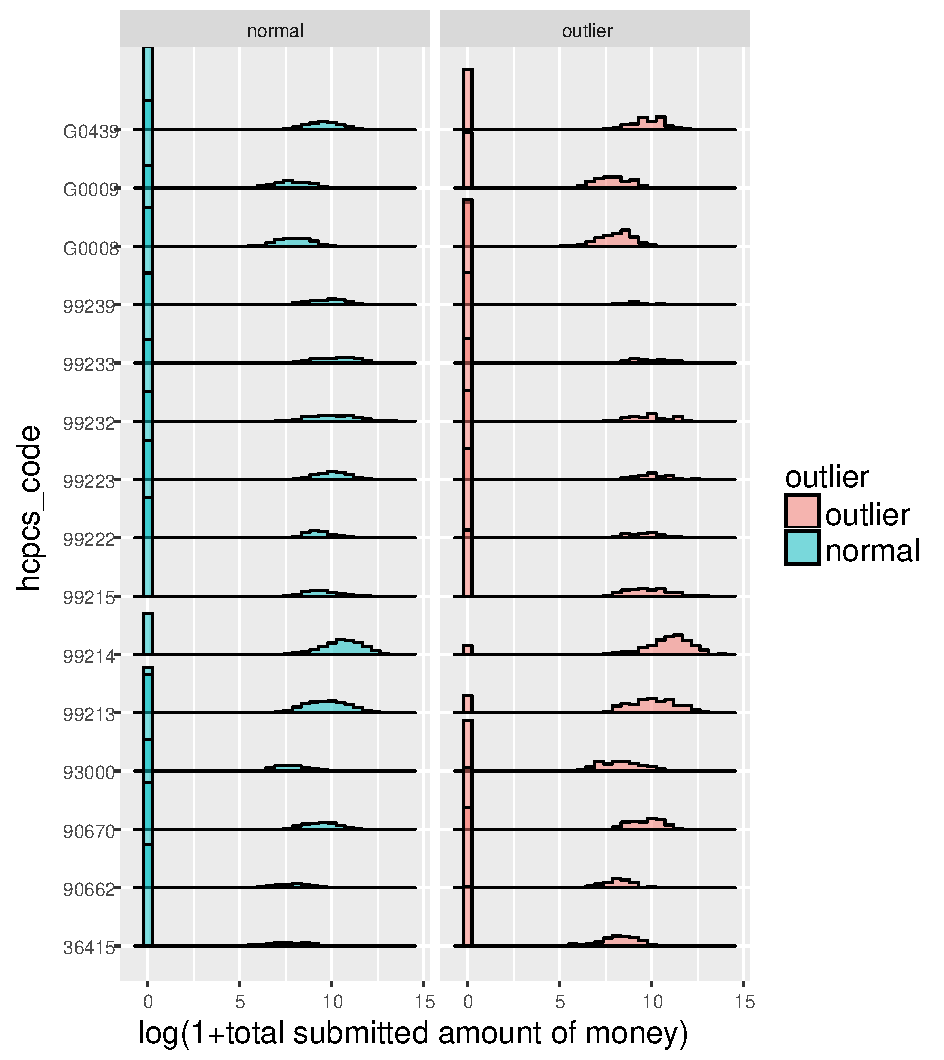
\includegraphics[scale=0.6]{../img/Dist-out-amount.pdf}}
\caption{Histograms of log-transformed submitted charged amount of money of top 15 most claimed services with regard to their outlier labels. HCPCS code: 
99213 is established patient office or other outpatient visit, typically 10 minutes, 99214 is established patient office or other outpatient visit, typically 15 minutes and  99215 is established patient office or other outpatient visit, typically 40 minutes. We can see this outlier provider has smaller 99213 amount and higher 99215 amount than normal providers. This may indicate that we could find the up-coding fraud.  Up-coding means billing more costly services than the one actually performed.}
\label{fig:dev-out-amt}
\end{figure}

\begin{figure}[H]
\centerline{\includegraphics[scale=0.4]{../img/Outlier-map.pdf}}
\caption{Regional distribution of health care receipts. X-axis shows the longitude and Y-axis shows the latitude of providers. Red circles represent outliers detected by the proposed method, and  blue circles others. The radius of circle corresponds to the number of providers.}
\label{fig:out-map}
\end{figure}

As a typical example, \Figref{fig:outlier} shows log-transformed submitted charged amount of money of top 15 most claimed service of outlier providers(npi code is 1134298938) and histogram of that of normal providers. Red points shows the outlier. We can see this provider has smaller 99213 amount and higher 99215 amount than mean of normal providers. This may also indicate that we could find provider that committed the up-coding fraud.  


\begin{figure}[H]
\centerline{\includegraphics[scale=0.42]{../img/Outlier.pdf}}
\caption{Typical example of submitted amount of money of outlier. Red points represent submitted amounts of money for provider detected as outliers, and blue bars represent histogram of that of normal providers.}
\label{fig:outlier}
\end{figure}

\end{comment}

LOF with the data-split: PROVIDER and feature: HCPCS has the best AUC score. Here we see more detail result of the model and matches between outliers and frauds.
\Tabref{tb:auc-provider} shows the AUC scores by the provider types. We see several providers who commit fraud. The AUC score of Neurosurgery is the highest. 
The NPI code of the provider who committed fraud is 1003904830. His score gets top 3 score out of 441 Neurosurgery providers. \Figref{fig:Neuro} shows the histograms of the submitted amount of 
money on each HCPCS procedure in Neurosurgery and submitted amount of money with NPI code, 1003904830. He submitted most for these four HCPCS codes.
\Figref{fig:Neuro} shows that he submitted more than normal providers with these HCPCS codes and this can be a sign of fraud. 
Next, in the case of Diagnostic Radiology, the NPI code of provider who committed fraud is 1619117538. His outlier score was top 294 out of the 4298 diagnostic radiology providers.
News reports that he wrote more than 250 illegal prescriptions over a four-year period, starting in 2010, for Oxycodone, Percocet and, Hydrocodone\cite{Diagnostic}. 
\Figref{fig:Diagnostic} shows the histograms of the submitted amount of money on each HCPCS procedure in Diagnostic Radiology and submitted amount of money with NPI code, 1619117538.
His records of submission do not record high amounts for these kinds of operations, though he gets higher outlier score than other diagnostic radiology providers. We think that there are two possible reasons for the illegal activities not being recorded in the datasets.
First, the illegal submission procedure is not included in the Medicare program. Second, this illegal operation was stopped before 2015 and were not recorded in our dataset. We cannot explain why he gets high outlier score from the histograms of his submission amounts.
\par



\input{../data/AUC-Provider.tex}

\begin{figure}[H]
	\begin{tabular}{cc}
	\begin{minipage}{.5\hsize}
	\centering
	\centerline{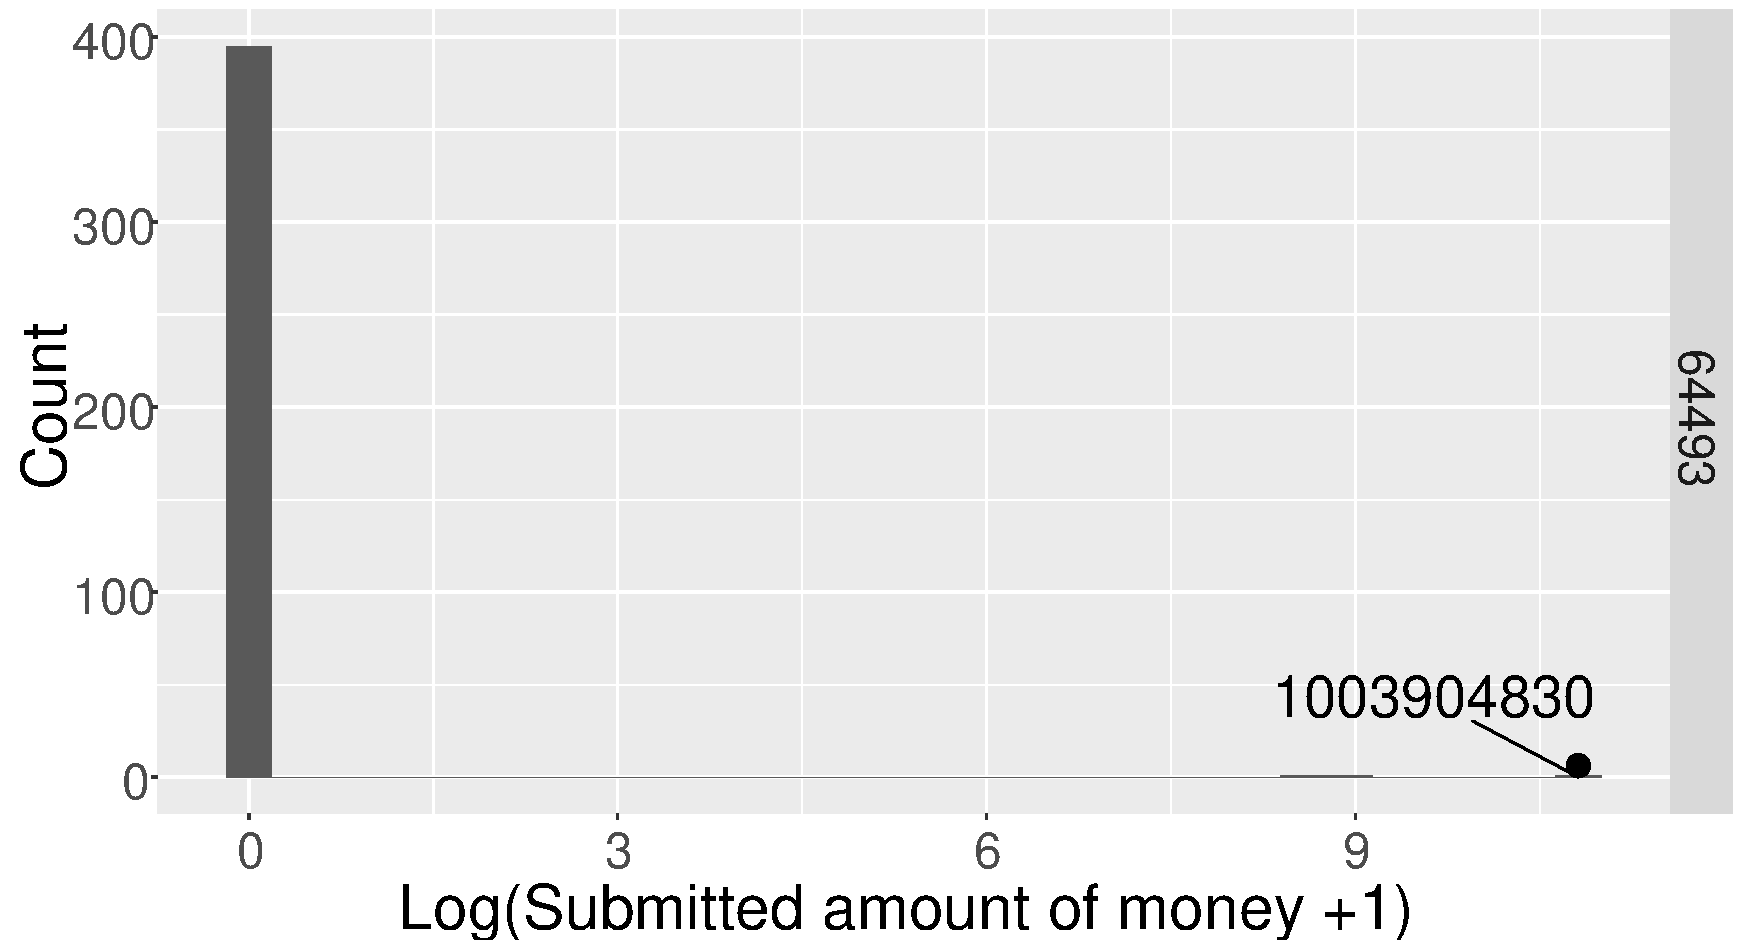
\includegraphics[scale=0.22]{../img/fraud/Neurosurgery-64493.pdf}}
%	\subcaption{Histogram of log of total submitted amount of money of providers whose speciality is internal medicine.}
	\subcaption{}\label{fig:Neuro1}
	\end{minipage} 
      %---- 2番目の図 --------------------------
      \begin{minipage}{.5\hsize}
        \centering
        \centerline{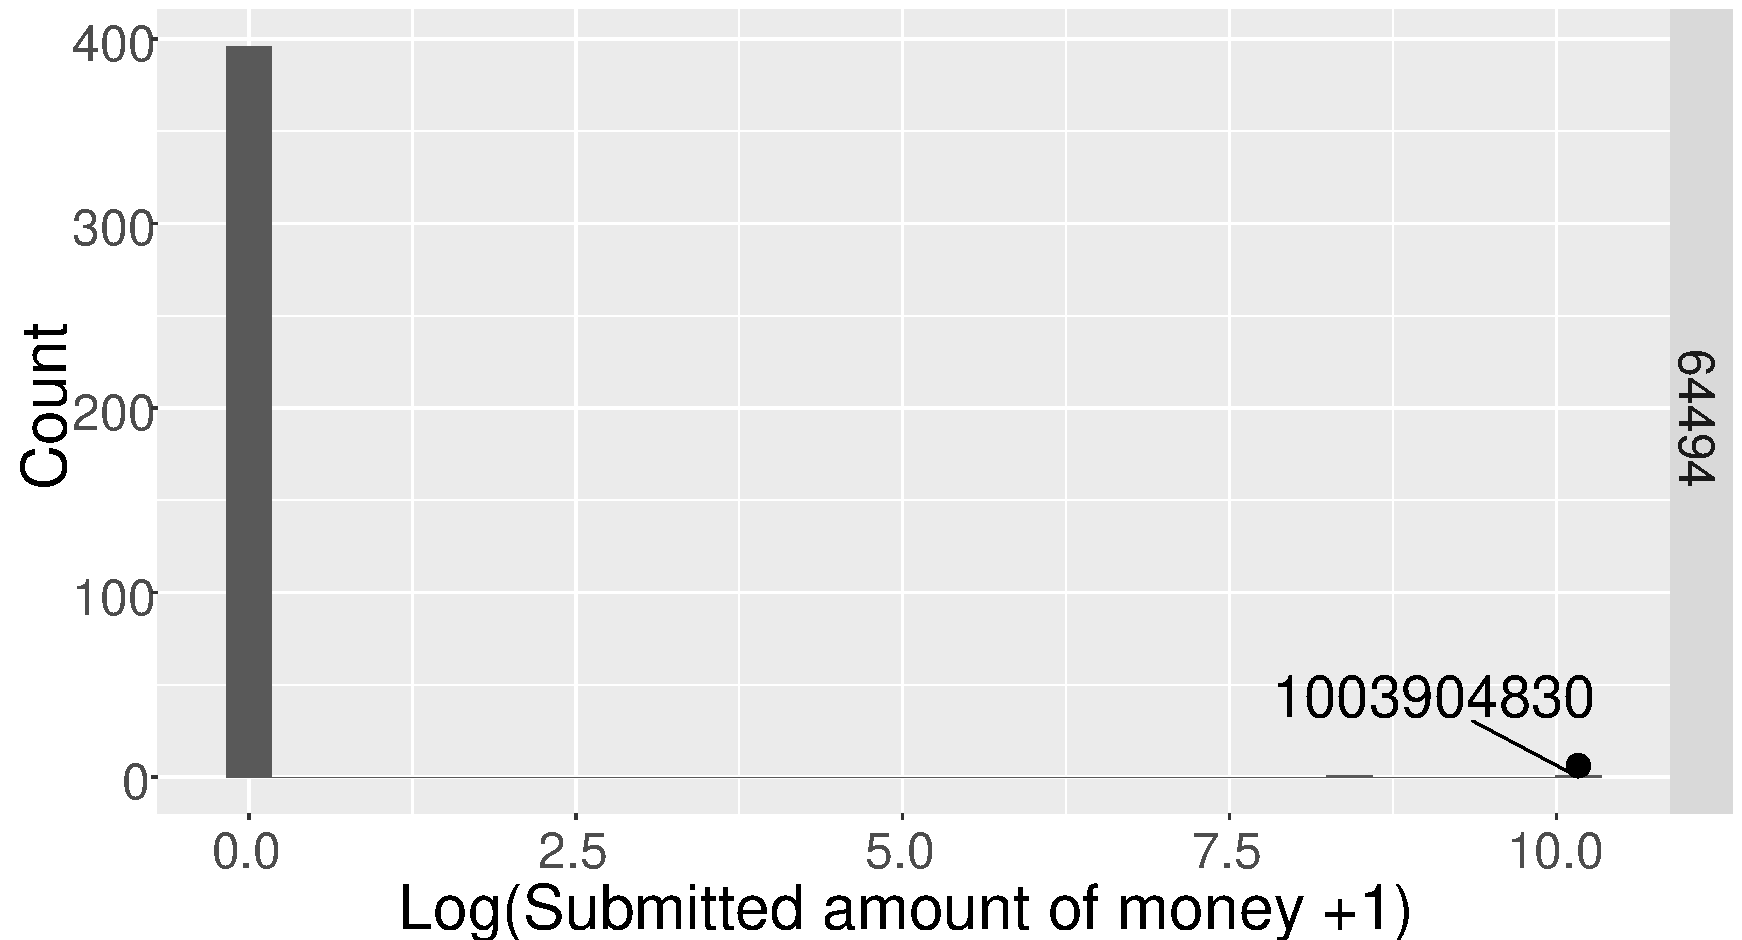
\includegraphics[scale=0.22]{../img/fraud/Neurosurgery-64494.pdf}}
%        \subcaption{Histogram of log of total submitted amount of money of providers whose speciality is peripheral vascular disease.}
	\subcaption{}\label{fig:Neuro2}
      \end{minipage} \\
      %---3番目の図---------
       \begin{minipage}{.5\hsize}
        \centering
        \centerline{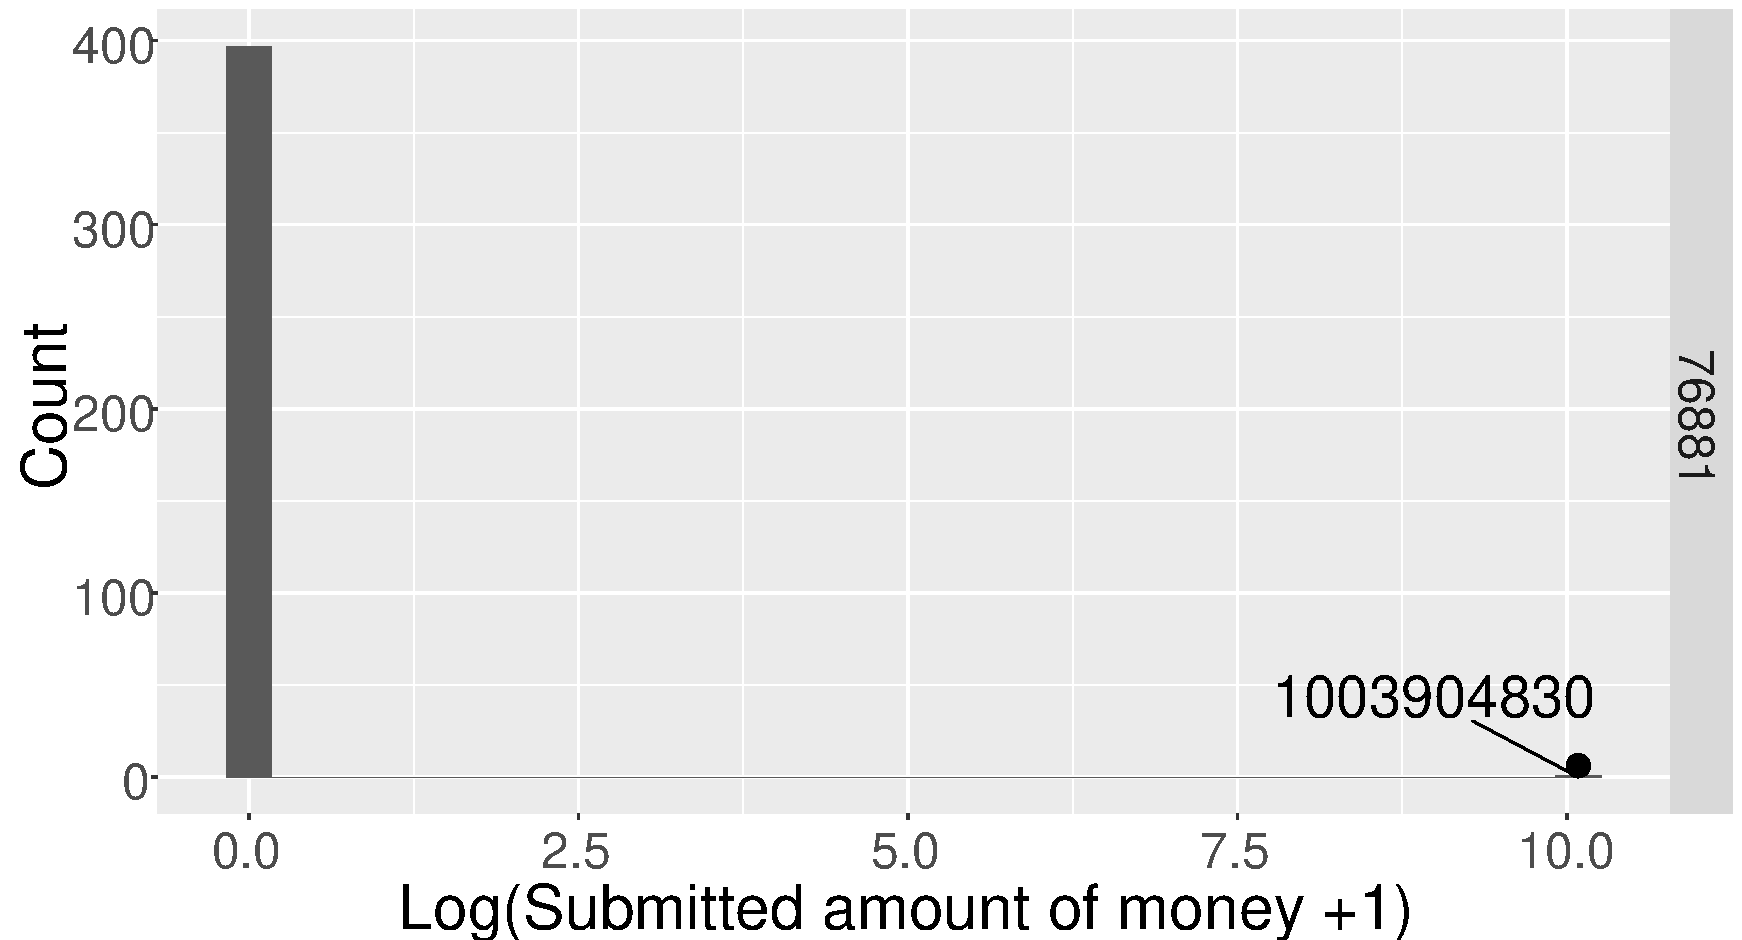
\includegraphics[scale=0.22]{../img/fraud/Neurosurgery-76881.pdf}}
%        \subcaption{Histogram of log of total submitted amount of money of providers whose speciality is addiction medicine.}
	\subcaption{}\label{fig:Neuro3}
      \end{minipage} 
      %----4番目の図---------
       \begin{minipage}{.5\hsize}
        \centering
        \centerline{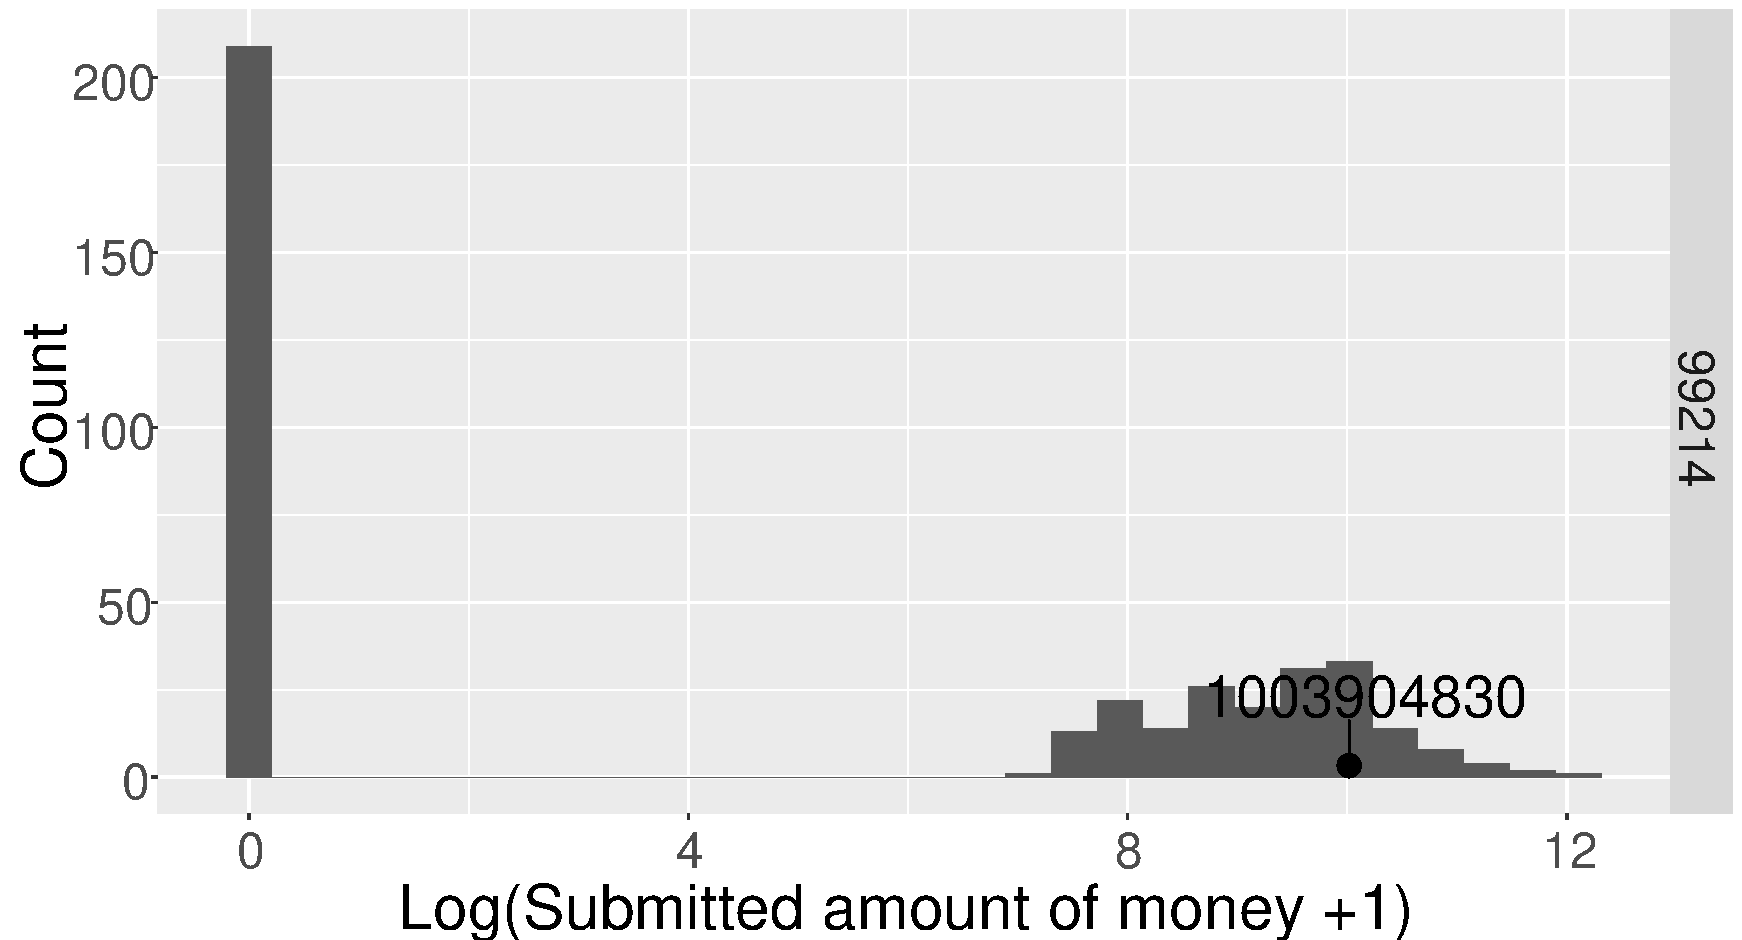
\includegraphics[scale=0.22]{../img/fraud/Neurosurgery-99214.pdf}}
%        \subcaption{Histogram of log of total submitted amount of money of providers whose speciality is certified nurse midwife.}
	\subcaption{}\label{fig:Neuro4}
      \end{minipage} \\
      %---- 図はここまで ----------------------
    \end{tabular} 
     \caption{\subref{fig:Neuro1} depicts histogram of $\log (\mbox{total submitted amount of money} +1)$ of HCPCS code, 64493(Injections of lower or sacral spine facet joint using imaging guidance) of Neurosurgery providers and the value of fraudulent providers. 
     \subref{fig:Neuro2} depicts that of HCPCS code 64494 (Injections of lower or sacral spine facet joint using imaging guidance). 
     \subref{fig:Neuro3} depicts that of HCPCS code 76881 (Ultrasound of leg or arm).
     \subref{fig:Neuro4} depicts that of HCPCS code 99214 (Established patient office or other outpatient, visit typically 25 minutes). He submitted more than normal providers with these HCPCS codes and this can be a sign of fraud. }
      \label{fig:Neuro}
\end{figure}



\begin{figure}[H]
	\begin{tabular}{cc}
	\begin{minipage}{.5\hsize}
	\centering
	\centerline{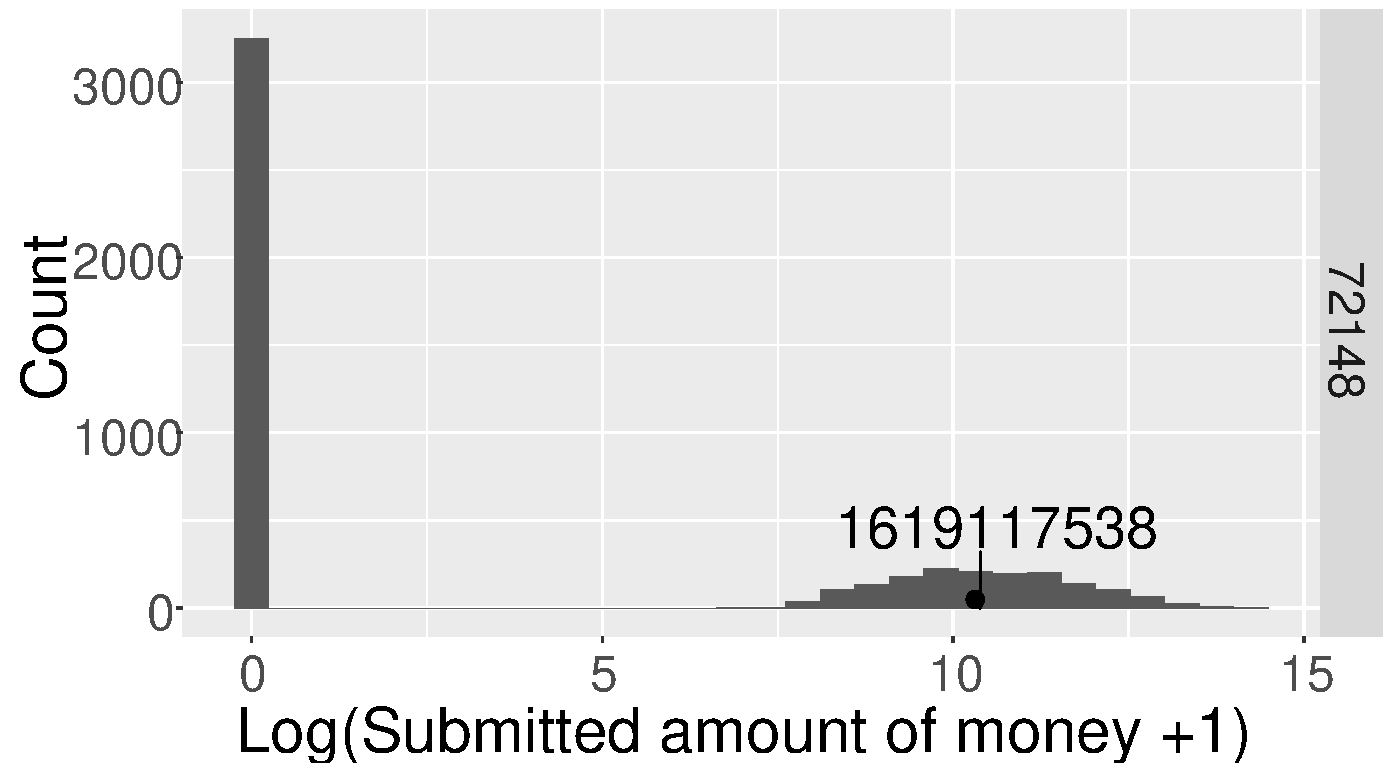
\includegraphics[scale=0.22]{../img/fraud/Diagnostic-Radiology-72148.pdf}}
%	\subcaption{Histogram of log of total submitted amount of money of providers whose speciality is internal medicine.}
	\subcaption{}\label{fig:Diagnostic1}
	\end{minipage} 
      %---- 2番目の図 --------------------------
      \begin{minipage}{.5\hsize}
        \centering
        \centerline{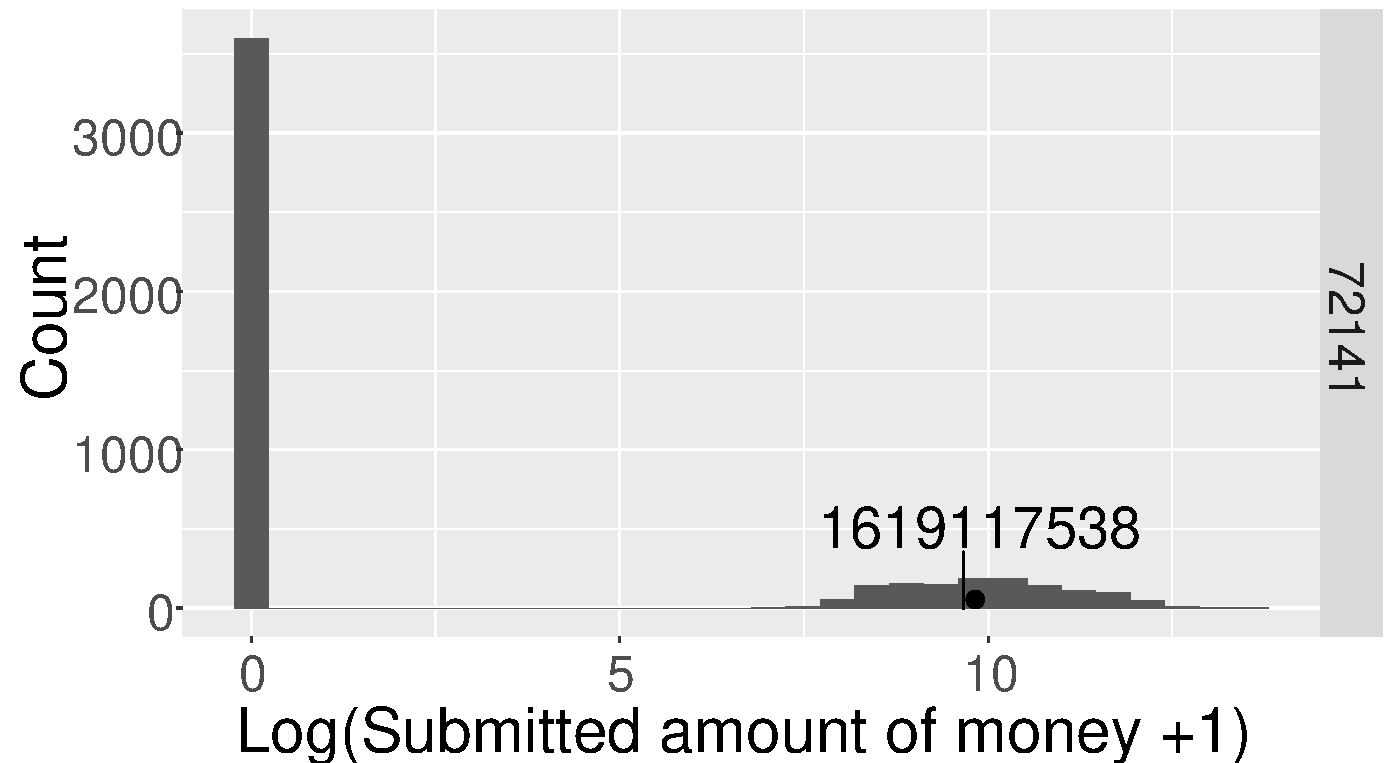
\includegraphics[scale=0.22]{../img/fraud/Diagnostic-Radiology-72141.pdf}}
%        \subcaption{Histogram of log of total submitted amount of money of providers whose speciality is peripheral vascular disease.}
	\subcaption{}\label{fig:Diagnostic2}
      \end{minipage} \\
      %---3番目の図---------
       \begin{minipage}{.5\hsize}
        \centering
        \centerline{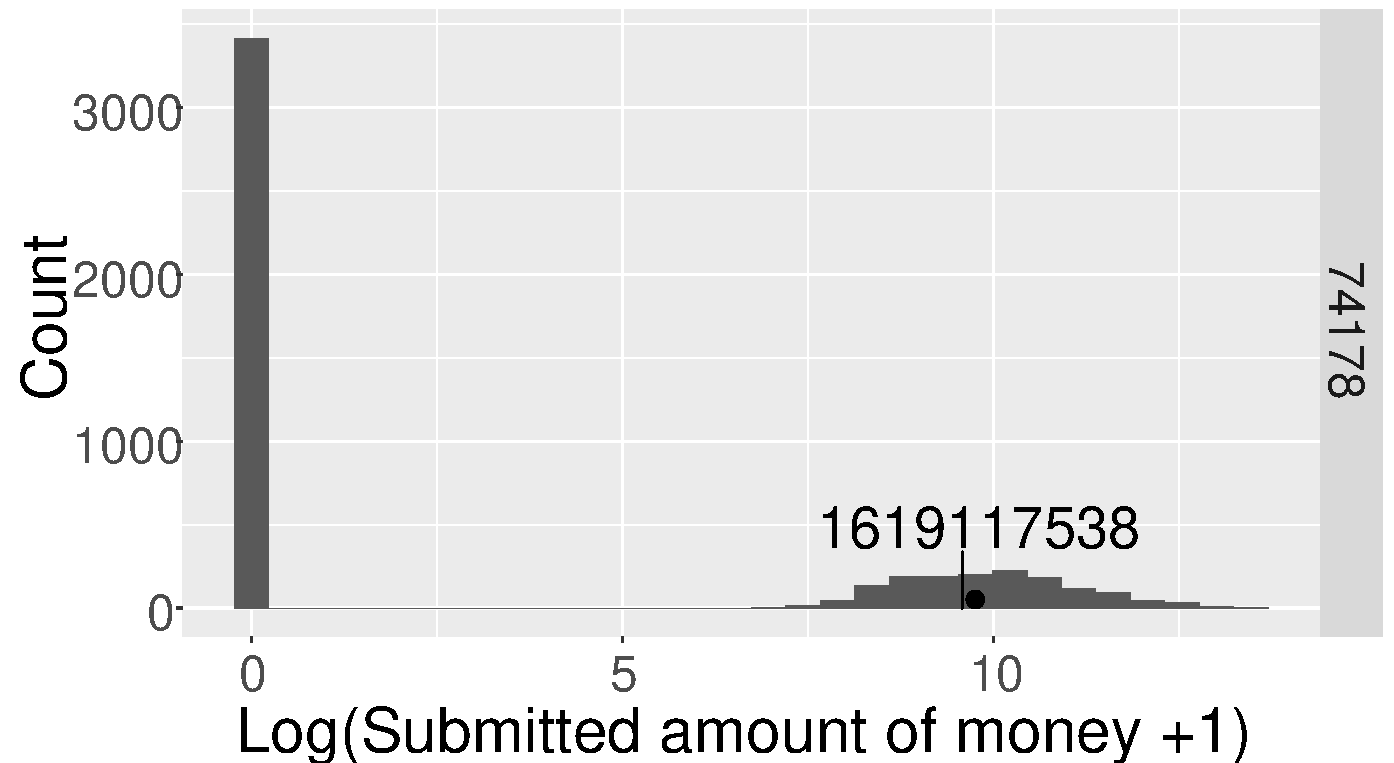
\includegraphics[scale=0.22]{../img/fraud/Diagnostic-Radiology-74178.pdf}}
%        \subcaption{Histogram of log of total submitted amount of money of providers whose speciality is addiction medicine.}
	\subcaption{}\label{fig:Diagnostic3}
      \end{minipage} 
      %----4番目の図---------
       \begin{minipage}{.5\hsize}
        \centering
        \centerline{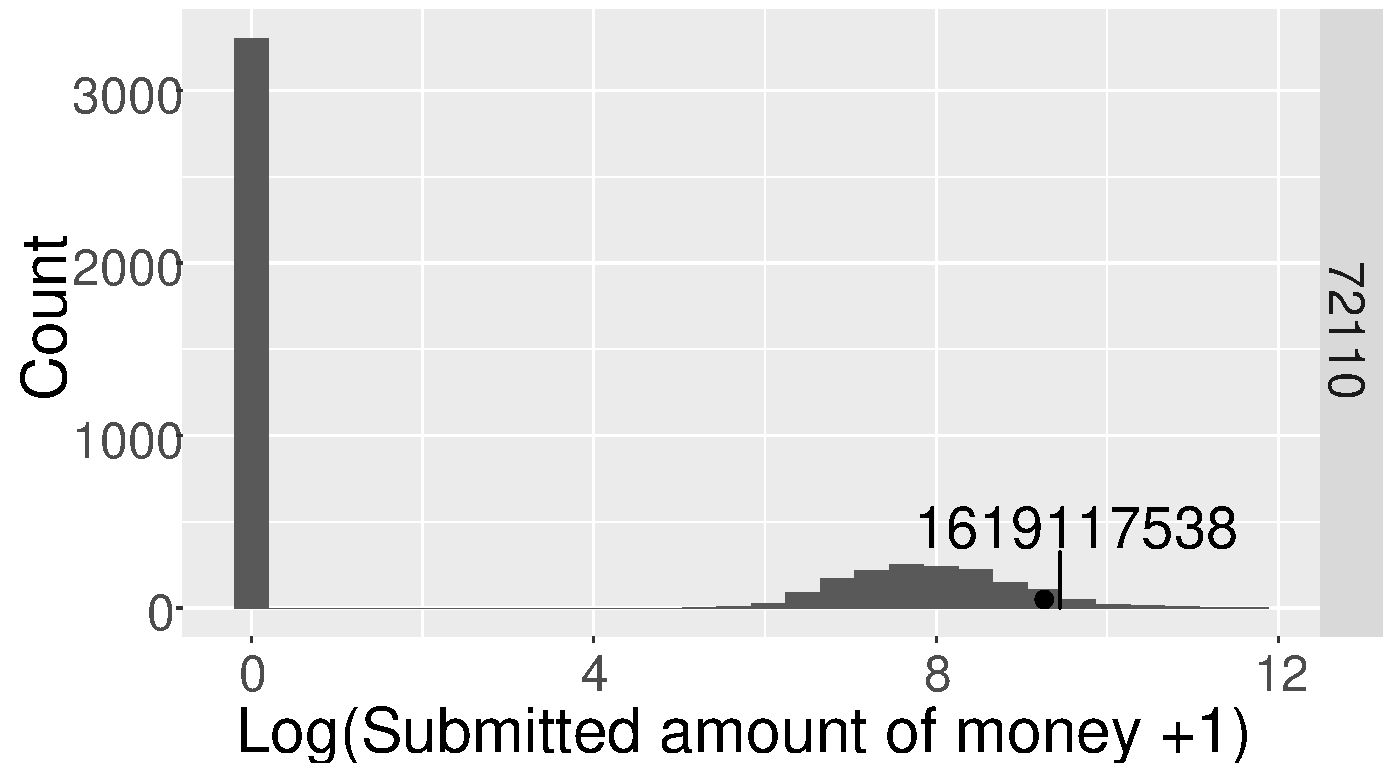
\includegraphics[scale=0.22]{../img/fraud/Diagnostic-Radiology-72110.pdf}}
%        \subcaption{Histogram of log of total submitted amount of money of providers whose speciality is certified nurse midwife.}
	\subcaption{}\label{fig:Diagnostic4}
      \end{minipage} \\
      %---- 図はここまで ----------------------
    \end{tabular} 
   
     \caption{\subref{fig:Diagnostic1} depicts histogram of $\log (\mbox{total submitted amount of money} +1)$ of HCPCS code, 72148(MRI scan of lower spinal canal) of Neurosurgery providers and the value of fraudulent providers. 
     \subref{fig:Diagnostic2} depicts that of HCPCS code 72141 (MRI scan of upper spinal canal). 
     \subref{fig:Diagnostic3} depicts that of HCPCS code 74178 (CT scan of abdomen and pelvis before and after contrast).
     \subref{fig:Diagnostic4} depicts that of HCPCS code 72110 (X-ray of lower and sacral spine, minimum of 4 views.) We cannot explain why he gets high outlier score from the histograms of his submission amounts.}
      \label{fig:Diagnostic}
\end{figure}
\par
We evaluated whether outliers and frauds are matched in the healthcare insurance claims. However, the score in other domain can be different from the Medicare cases. We applied One-SVM and LOF to credit card fraud detection.
Actually, the performance of credit card fraud detection is different from the medicare cases. One-SVM outperformed LOF and the score is significantly high. The result of is not different from random extraction. This implies that 
the detection performance, matches between fraud and outlier, is determined not only by detection algorithm but also data features.


\subsection{Ratio of the outliers in One-SVM}
Next, we changed hyperparameter $\nu$ of One-SVM at 20 points from 0.001 to 0.98. \Figref{fig:nu} shows the ratio of outliers on various $\nu$.
As we expected, we can easily see as $\nu$ increases, the ratio of the outliers also increases. Thus, we can regulate the ratio of the outliers by changing $\nu$.
\begin{figure}[H]
\centerline{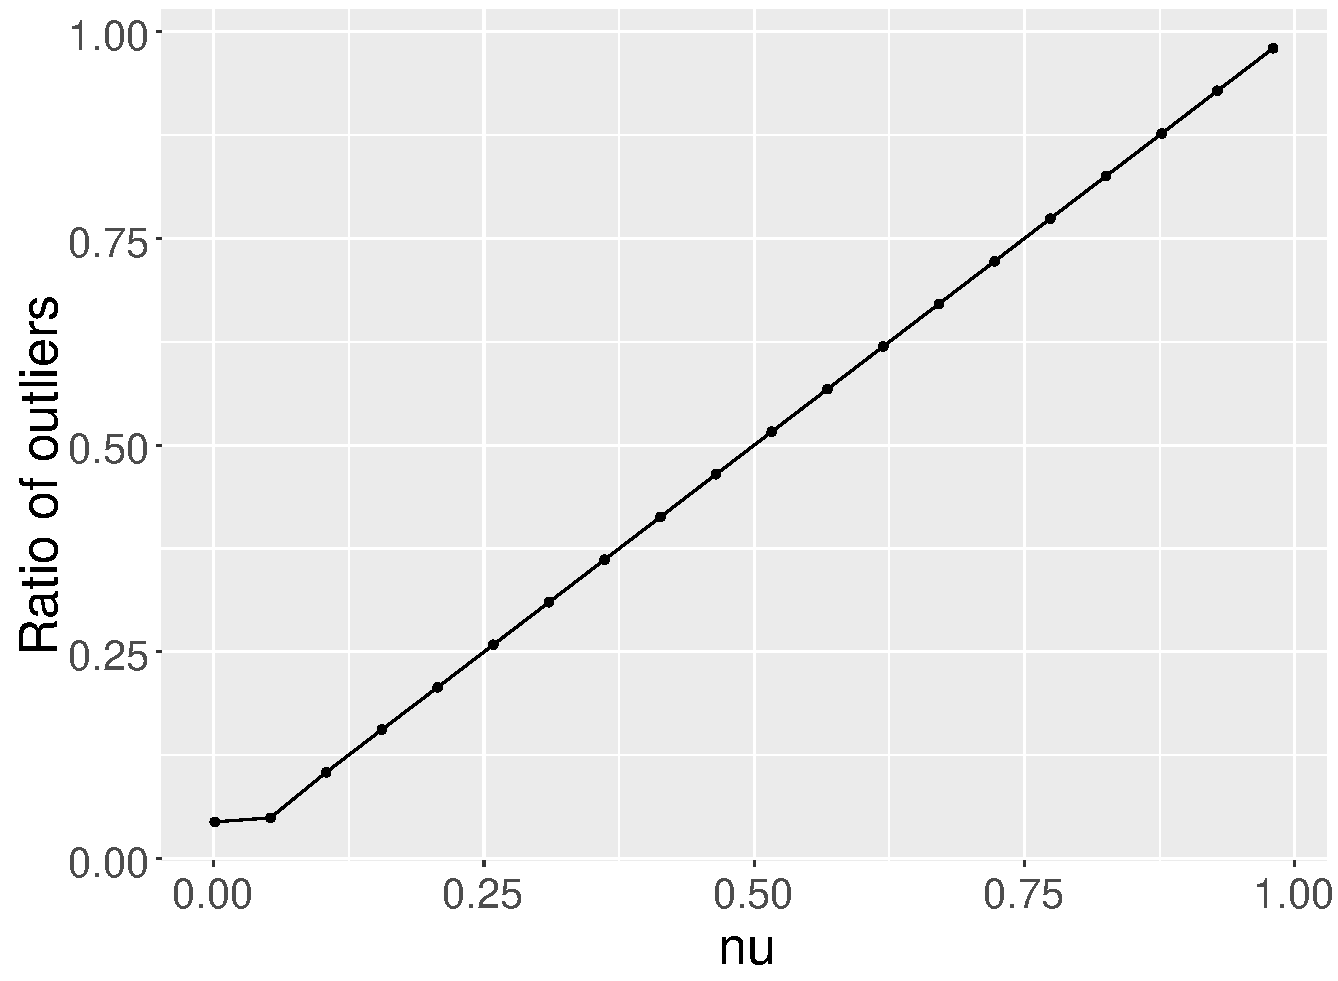
\includegraphics[scale=0.32]{../img/ratio-of-outliers.pdf}}
\caption{Ratio of the outliers in terms of  $\nu$. x axis shows the hyperparameter $\nu$ which is an upper bound of the ratio of the outliers and y axis shows
the ratio of outlier detected by One-SVM of which $\nu$ = $x$.}
\label{fig:nu}
\end{figure}


\section{Conclusions}\label{sec:conclusions}
We applied data linkage methods to the NPI, Healthcare Provider Taxonomy Core, and zip code. We used world grid square codes to segment regions regarding physicians' geospatial heterogeneities and investigated world grid square statistics about the submitted amount of money and the provider type variance. We applied One-SVM and LOF to the feature vectors, HCPCS: submitted amount of money for each HCPCS code and STAT: summary statistics of the submitted amount for money and one-hot encoding of physicians'  characteristics. By dividing large records based on physicians' locations using world grid square codes and types into many segments, we obtained many small datasets about the healthcare receipts. Finally, we evaluated the method using LEIE labels. 
LOF performs better than One-SVM. LOF with data-split: Provider and feature: HCPCS is the best of all methods. Data-split is also beneficial in terms of the time of calculation.
\par
As future work, first, as we see in the design of feature vectors and their performance, the feature engineering is crucial when we define the fraud claims in the health care receipts. We may need deep knowledge of the healthcare domain in order to select effective features.
Second, we should interview healthcare fraud subject matter experts whether providers with higher outlier scores are fraudulent. Some providers who are not in LEIE datasets, but have high outlier score may be the real fraudulent providers.
Third, the tradeoff between the true positive rate and the false positive rate should be adjusted. If we allow only low true positive rates, then  there are more rooms for benefits by increasing the cost of the experts who find the providers actually committing fraud from fraudulent cases in order to prevent them from receiving money. On the other hand, if we allow a high true positive rate, the cost of the experts increases, and the costs are higher than the money given to the providers who commit fraud. 
Fourth, more sophisticated datasets are needed. We used Medicare Provider Utilization and Payment Data, Full Replacement Monthly NPI in 2015 and List of Excluded Individuals after 2015. However, if their exclusion resulted from illegal activities before 2015, then their illegal activities are not recorded in the Provider Utilization and Payment Data, Full Replacement Monthly NPI and List of Excluded Individuals includes providers. In addition List of Excluded Individuals include providers who were excluded not only for their fraud-related activities but for their other illegal activities such as physical contact with their patients. Thus, more sophisticated datasets that record provider activities and frauds related to these activities are needed.

%\bibliography{conference} %bibファイルの.bibの前の部分
%\bibliographystyle{unsrt} %引用された順番に出力



%%% Acknowledgments %%%%%%%%%%%%%%%%%%%%%%%%%%%%%%%%%%%%%%%%%%%%%%%%%%%%%%%%%%%%%
\acknowledgment
The author would like to express his sincere gratitude to Associate Professor
Aki-Hiro Sato for his helpful advices and appreciate the feedback offered by Professor Ken Umeno.

%%% References %%%%%%%%%%%%%%%%%%%%%%%%%%%%%%%%%%%%%%%%%%%%%%%%%%%%%%%%%%%%%%%%%%
%%% If you want to use BibTeX, delete the above and insert code here.
%% \bibliographystyle{...}
%% \bibliography{...}
\Urlmuskip=0mu plus 1mu\relax
\bibliographystyle{unsrt} %引用された順番に出力
\bibliography{conference} %bibファイルの.bibの前の部分

%%% Appendix %%%%%%%%%%%%%%%%%%%%%%%%%%%%%%%%%%%%%%%%%%%%%%%%%%%%%%%%%%%%%%%%%%%%
%%% If you don't need appendices, delete the below.
\appendix

\section{Appendix}

\subsection{World Grid Square Code}\label{sec:world-grid-square-code}
World grid square code\cite{ASatoMesh} is an extension of  the Japanese Industrial Standard (JIS) for gird square codes (JIS X0410 \cite{MeshJIS}) established in 1976.
World grid square code is defined from 1\--st grid square code to 6 \--th grid square code. However we only used 1\-- st grid square code. Here, we give the definition of 1\--st world grid square code.
See \cite{ASatoMesh} for more details. Firstly, we define three binary variable $x,y,z$ to separate the earth into eight areas based on latitude and longitude and construct 0\--th level gird square code.
The three variables are given as follows:
\begin{flalign}
x  & = \begin{cases}
	0  &\mbox{(if latitude is positive)}\\
	1 & \mbox{(otherwise)}
\end{cases}, \\
y  & = \begin{cases}
	 0 & \mbox{(if longitude is positive)} \\
	 1 & \mbox{(otherwise)}
\end{cases}, \\
z & = \begin{cases}
	0 & \mbox{(if} \mid \mbox{longitude} \mid < 100^{\circ} \mbox{)} \\
	1 & \mbox{(otherwise)}
\end{cases}.
\end{flalign}
We define the 0\--th level grid square code $o$ as 
\begin{align}
	o = 2^{2}x + 2y + z + 1.
\end{align}
The 1\-- st grid square code can be calculated by 
\begin{align}
1 \mbox{\-- st grid square code} = 
\begin{cases}
	o00p0u & (p < 10, u < 10)\\
	o0p0u &(10 \leq p < 100, u < 10)\\
	op0u &(100 \leq p, u < 10)\\
	o00pu & (p < 10, 10 \leq u)\\
	o0pu &(10 \leq p < 100, 10 \leq u)\\
	opu &(100 \leq p, 10 \leq u)
\end{cases},
\end{align}
where $p$ and $u$ are defined as
\begin{align}
p &:= \lfloor(1-2x) \mbox{latitude} \times 60 \div 40 \rfloor ,&\\
u &:= \lfloor(1-2y) \mbox{longitude} -100z \rfloor & \mbox{($u$ is one or two digits)}.
\end{align}
For example, latitude is 35.010348 and longitude is 135.768738, then 1 \--st grid square code is 105235.





%\subsection{Providers' Specialities and their taxonomy codes}\label{sec:specialities}
%We split data by their speciality and their location. Here we show the specialities and their taxonomy codes\cite{Taxonomy}. 
%\Tabref{tb:taxonomy} shows the providers' speciality and their taxonomy codes.
%We split data by their speciality and their location. Here we show the specialities\cite{Taxonomy}.
%Specialities have 141 kinds.
%\input{../data/provider-discription.tex}
%\input{../data/taxonomy.tex}






\subsection{Outlier detection to extract credit card fraud}\label{sec:credit-card}
In this section, we apply outlier detection techniques to another domain, Credit card fraud detection\cite{CreditCard}. This dataset is composed of credit card transactions from September 2013.
It contains a subset of online transactions that occurred in two days, where we have 492 frauds out of 284,807 transactions. It consists of 31 columns, where Time column denotes the second
elapsed between each transaction and the first transaction in the dataset, Amount column denotes the transaction, Class column takes 1 in case of fraud and 0 otherwise and the meanings of
remaining columns are not revealed for confidentiality reason and the features have been transformed by means of principal components. 
%The computational time is long if we apply outlier detection algorithms to all data points. We randomly sample 492 frauds and 99508 normal transactions. 
Excluding Time and Class columns, the feature vectors are made. \Listref{pro:1} shows the program of outlier detections and their evaluations. \Figref{fig:credit-roc} shows the roc curve of the two models. 
\Tabref{tb:credit-auc} shows the AUC score of the two models. Contrary to the fraud detection of medicare transaction, One-SVM performs well and LOF performs worse and is below random
sampling.

\begin{table}[htb]
\centering
  \caption{AUC score of the two outlier detection models for credit transaction fraud detection.}
  \begin{tabular}{lr} \hline \hline
    Outlier Detection Model  & AUC \\ \hline
    LOF &  0.506 \\
    One-SVM &  0.942\\ \hline
   \end{tabular}
  \label{tb:credit-auc}
 \end{table}



\begin{figure}[H]
\centerline{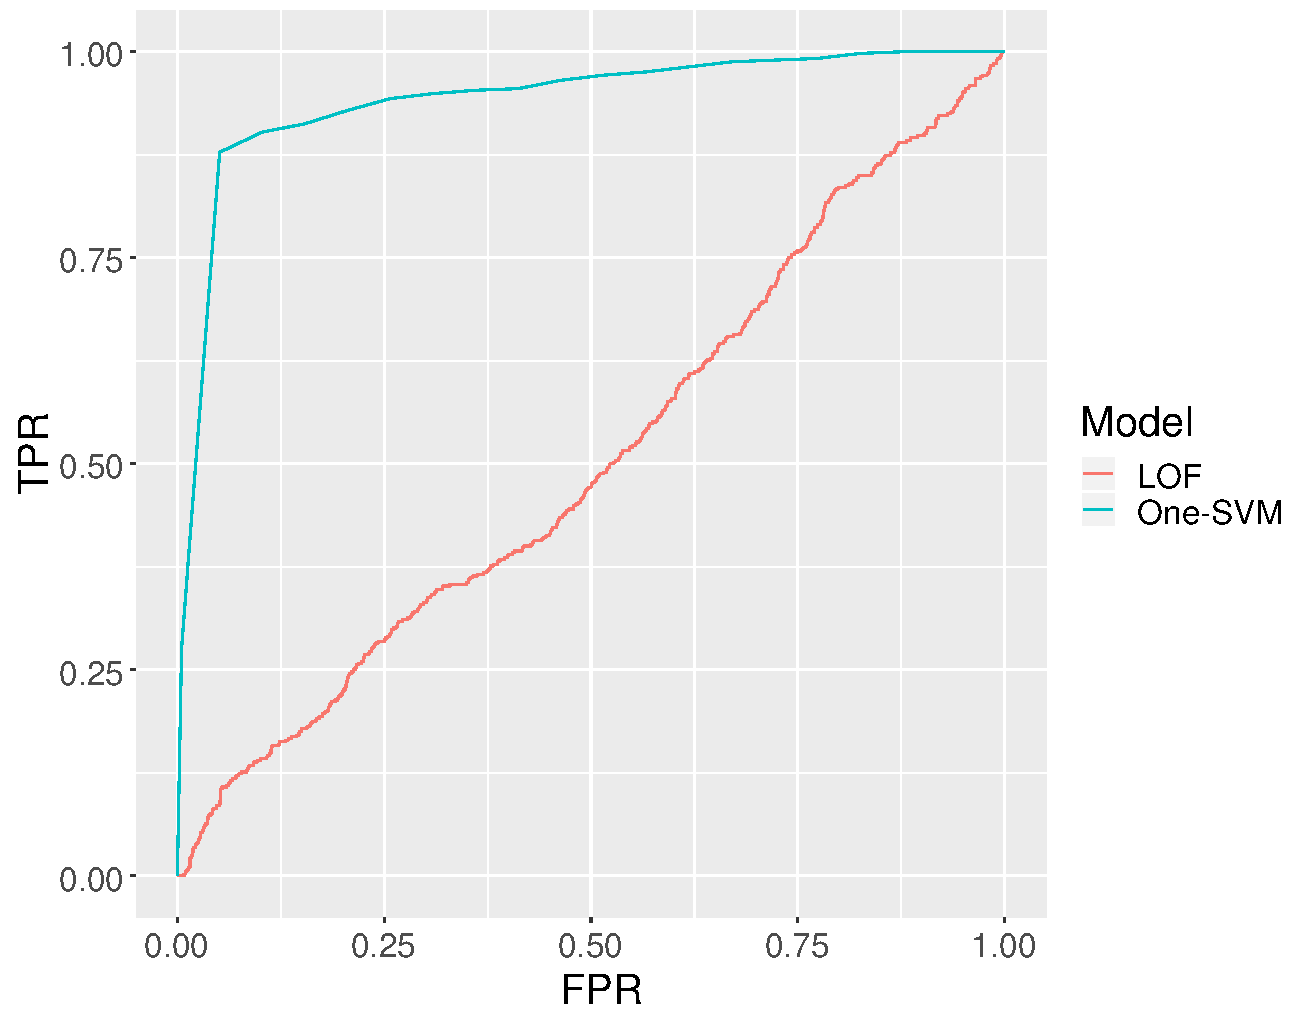
\includegraphics[scale=0.5]{../img/credit-roc.pdf}}
\caption{ROC curves of the LOF and One-SVM. Model shows the type of outlier detection methods. One-SVM outperforms LOF.}
\label{fig:credit-roc}
\end{figure}


\lstinputlisting[caption = The code for outlier detection. ,label = pro:1]{../script/script/credit-for-tex.R}


\begin{comment}
\subsection{Outlier detection to GRIDSTATS}\label{sec:outlier-meshstats}
We applied outlier detection technique : LOF to GRIDSTATS. We expect that some geographically abnormal places are found.
\Figref{fig:outlier-meshstats} shows the result of the outlier detection. The red rectangles shows the mesh which was detected as outlier and the blue rectangles shows the normal mesh.
We can see that meshs which has no people such as meshes in the lake BIWA and meshes in the mountains are detected as outlier and meshes which is very crowded such as 
meshes around the Karasuma station and Kawaramachi station are detected as outlier. 

\begin{figure}[H]
\centerline{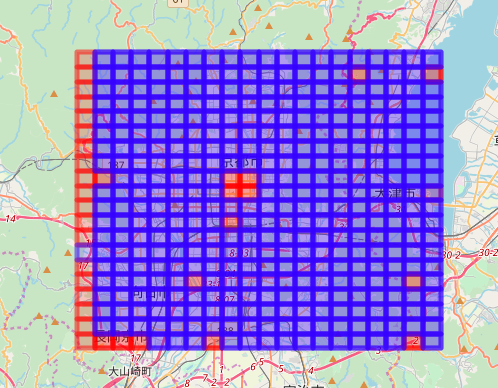
\includegraphics[scale=0.42]{../img/outlier-meshstats.png}}
\caption{Map around Kyoto-City. The red rectangles shows the mesh which was detected as outlier and the blue rectangles shows the normal mesh. We can see that meshs which has no people such as meshes in the lake BIWA and mesh}
\label{fig:outlier-meshstats}
\end{figure}
\end{comment}

\subsection{List of exclusions}\label{sec:exclusions}
Here, we show the all exclusion reasons. \Tabref{exclusion} shows the exclusion codes and their descriptions.
\input{../data/exclusion.tex}

%%% End of body %%%%%%%%%%%%%%%%%%%%%%%%%%%%%%%%%%%%%%%%%%%%%%%%%%%%%%%%%%%%%%%%%
\fi
\ifoutputcover
\evenclearpage
%%% Covers and abstract for submission %%%%%%%%%%%%%%%%%%%%%%%%%%%%%%%%%%%%%%%%%%
\makecover                      % Cover
\makespine[\numberofspines]     % Spine
\fi
\ifoutputabstractforsubmission
\makeabstractforsubmission      % Abstract for submission
\fi
\end{document}
